\documentclass[aps,prl,twocolumn,10pt,superscriptaddress,floatfix]{revtex4-2}

\usepackage{amsmath}
\usepackage{graphicx}
\usepackage{longtable}
\providecommand{\texorpdfstring}[2]{#1}

\graphicspath{{figures/}}

\begin{document}

\title{Supplemental Material: Yukawa screening derivation of the bond-valence rule}

\author{Michael L. Whittaker}
\affiliation{Energy Geosciences Division, Lawrence Berkeley National Laboratory, Berkeley, CA 94720}
\affiliation{Materials Sciences Division, Lawrence Berkeley National Laboratory, Berkeley, CA 94720}
\author{Pan Wang}
\affiliation{Energy Geosciences Division, Lawrence Berkeley National Laboratory, Berkeley, CA 94720}
\author{Chunhui Li}
\affiliation{Meta Platforms, Inc., Menlo Park, CA 94025}
\author{Naman Katyal}
\affiliation{Energy Geosciences Division, Lawrence Berkeley National Laboratory, Berkeley, CA 94720}
\author{Piotr Zarzycki}
\affiliation{Materials Sciences Division, Lawrence Berkeley National Laboratory, Berkeley, CA 94720}

\maketitle

\onecolumngrid

\section{Data provenance}

The figures and tables in this Supplemental Material cover the same
103 cation--oxygen species analyzed in the main text, spanning $s$-,
$p$-, $d$-, and $f$-block cations.

Source structures are DFT-relaxed entries from the Materials Project.
For each structure, bond strengths were obtained by solving the
valence-sum and loop constraints on the cation--oxygen bond graph,
and $(R_0,B)$ were determined by linear least squares.  For
rank-deficient bond graphs (fewer independent bonds than parameters),
an anion-centered reparameterization was used; any remaining
ill-conditioned cases were resolved with the constrained nonlinear
procedure of Ref.~\citenum{Li2025}, with $R_0$ bounds $(-10,10)$~\AA.
Coordination numbers were determined from the bond graph.

The DFT-centroid comparison in Fig.~2 uses ten $s$-block oxides in
panel~a (Li$_2$O, Na$_2$O, K$_2$O, Rb$_2$O, Cs$_2$O, BeO, MgO, CaO,
SrO, and BaO) and 25 non-$s$-block oxides in panel~b: Al$_2$O$_3$,
SiO$_2$, GeO$_2$, SnO$_2$, PbO, TiO$_2$, V$_2$O$_5$, CoO, NiO, CuO,
ZnO, ZrO$_2$, MoO$_3$, PdO, Ag$_2$O, HfO$_2$, Ta$_2$O$_5$, Au$_2$O$_3$,
La$_2$O$_3$, Gd$_2$O$_3$, Yb$_2$O$_3$, B$_2$O$_3$, P$_2$O$_5$,
As$_2$O$_3$, and Sb$_2$O$_3$.  The panel-$b$ regression is defined
a priori as a test of the Yukawa screening picture only for
ground-state binary oxides whose cation environments approximate an
isotropic first-shell ionic screening cloud.  It therefore uses the 21
filled-symbol oxides and excludes B$_2$O$_3$, P$_2$O$_5$,
As$_2$O$_3$, and Au$_2$O$_3$, whose ground-state structures are dominated by
directional, non-isotropic bonding motifs; those four compounds are shown
as open symbols.  The 21 oxides shown as filled symbols in Fig.~2(b)
are the 25 listed above minus the four directional cases just named;
no further data-driven exclusion was applied beyond this fixed list.  The excluded oxides are the cases in this benchmark whose
ground-state cation environments are not compact first-shell ionic
polyhedra but directional or terminal-oxyanion motifs, so a single
shell centroid $m_i$ is not an adequate descriptor of the screening
cloud.

\section{\texorpdfstring{Coordination-number-resolved $B$--$R_0$ fit lines}{Coordination-number-resolved B-R0 fit lines}}

Figures~\ref{fig:group1_fits}--\ref{fig:fblock_fits_2} show the
$n$-resolved $B$ vs.\ $R_0$ fit lines for every species in the
103-cation set, grouped by block: Group~1 (Fig.~\ref{fig:group1_fits}),
Group~2 (Fig.~\ref{fig:group2_fits}), $3d$/$4d$/$5d$ transition metals
(Figs.~\ref{fig:dblock_fits_1}--\ref{fig:dblock_fits_8}), $p$-block
(Figs.~\ref{fig:pblock_fits_1}--\ref{fig:pblock_fits_3}), and $f$-block
lanthanides plus actinides
(Figs.~\ref{fig:fblock_fits_1}--\ref{fig:fblock_fits_2}).  Within each
coordination shell, the fitted parameters lie on a linear family
$B=\beta^{(n)}R_0+\beta_0^{(n)}$, and the lines converge toward
cation-specific characteristic pairs $(R_0^*,B^*)$ as described in the
main text.  Together, these atlas pages display every coordination-resolved
fit that contributes to the pole form $\beta=1/\ln(z/n)$ shown in
Fig.~1 of the main text.

\begin{figure}[t]
\centering
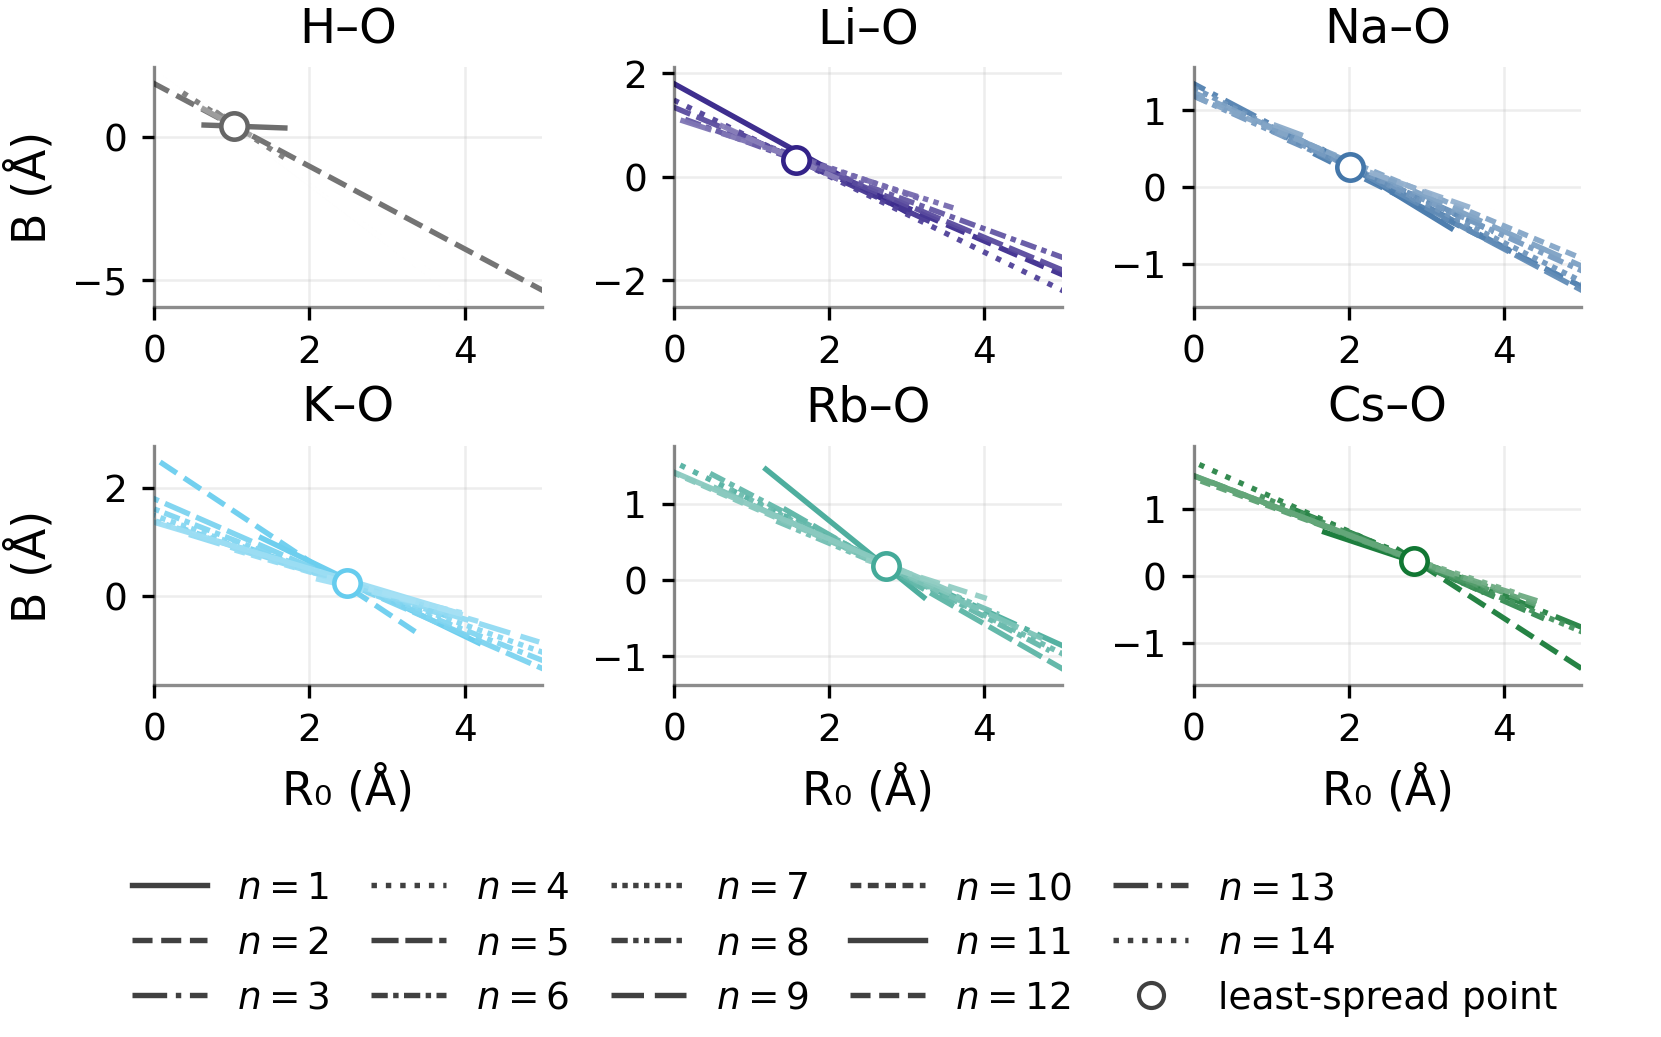
\includegraphics[width=0.85\textwidth]{group1_oxygen_cn_fit_lines.png}
\caption[Group~1 coordination-resolved $B$--$R_0$ lines.]{$n$-resolved $B$ vs.\ $R_0$ fit lines for Group~1 X--O pairs
(H, Li, Na, K, Rb, Cs).  Each colored line is a different coordination
number.  The convergence of the lines defines the characteristic pair
$(R_0^*,B^*)$ for each cation.}
\label{fig:group1_fits}
\end{figure}

\begin{figure}[t]
\centering
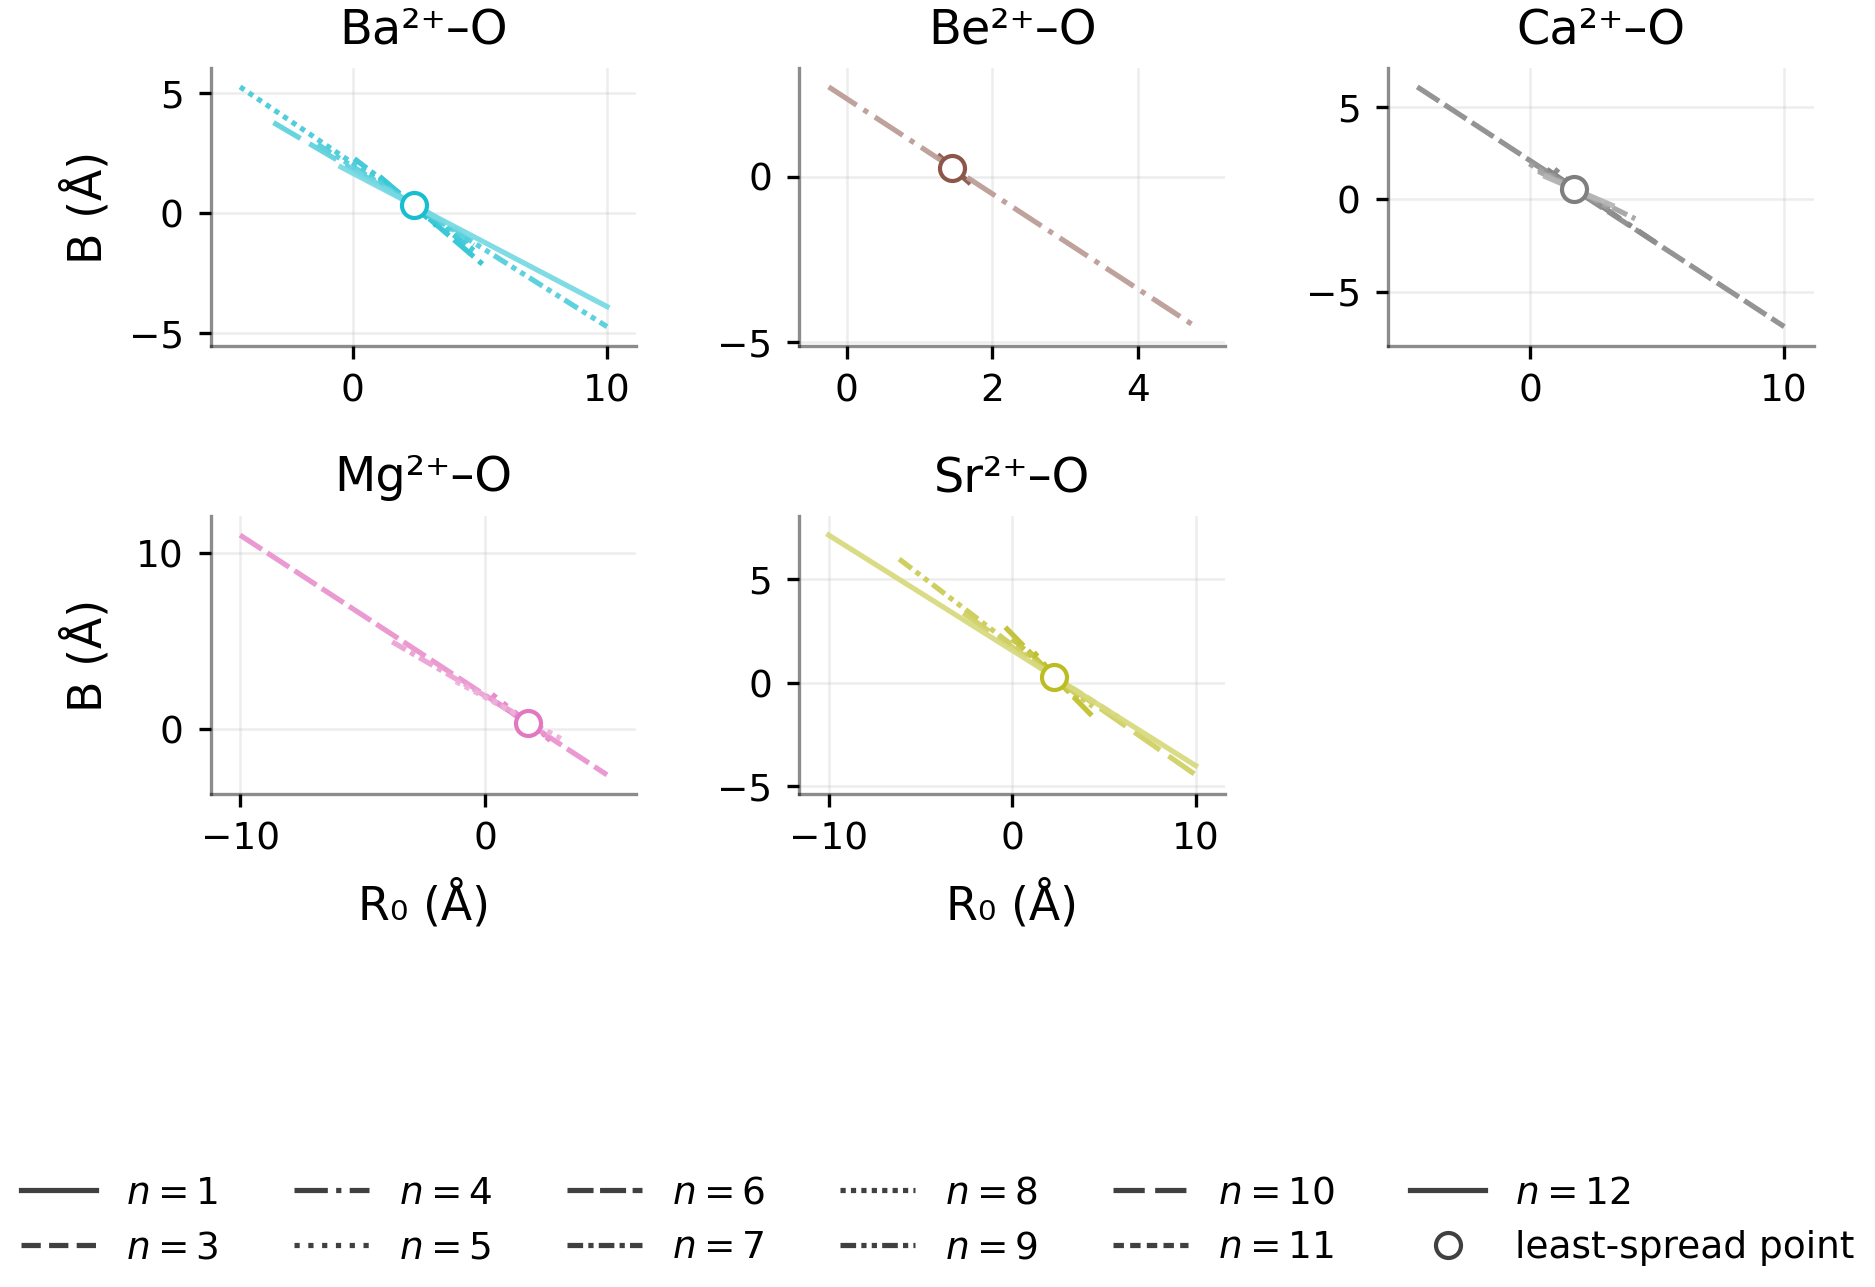
\includegraphics[width=0.85\textwidth]{group2_oxygen_cn_fit_lines_part01.png}
\caption[Group~2 coordination-resolved $B$--$R_0$ lines.]{$n$-resolved
$B$ vs.\ $R_0$ fit lines for Group~2 X--O pairs (Be, Mg, Ca, Sr, Ba).}
\label{fig:group2_fits}
\end{figure}

\paragraph*{Weighting scheme for the goodness-of-fit metrics.}
The weighted $R^2$ and mean absolute error reported with Fig.~1 of the
main text use weights $w_i=\max(N_i,1)$, where $N_i$ is the number of
DFT-relaxed structures contributing to the linear $B$--$R_0$ fit at
species $i$ and coordination $n$.  This gives more populous (species,
$n$) cells more leverage, in proportion to the number of independent
structures backing each fitted slope $\beta_i$.  Letting
$\hat\beta_i=1/\ln(z_i/n)$ be the parameter-free closed-form prediction
and $\bar\beta_w=\sum_i w_i\beta_i/\sum_i w_i$, the reported metrics are
\[
R^2_w
= 1 - \frac{\sum_i w_i\,(\beta_i-\hat\beta_i)^2}
            {\sum_i w_i\,(\beta_i-\bar\beta_w)^2},
\qquad
\mathrm{MAE}_w
= \frac{\sum_i w_i\,|\beta_i-\hat\beta_i|}{\sum_i w_i}.
\]
Pooling 68 species at $n=4$ ($\sum w=13{,}370$) with 82 species at
$n=6$ ($\sum w=17{,}162$) -- the $z\ne n$ subset shown in Fig.~1 --
gives $R^2_w=0.986$ and $\mathrm{MAE}_w=0.15$ for the parameter-free
closed form $\beta=1/\ln(z/n)$.  Per panel:
$R^2_w=0.973$, $\mathrm{MAE}_w=0.23$ at $n=4$; $R^2_w=0.979$,
$\mathrm{MAE}_w=0.089$ at $n=6$.

\paragraph*{Exclusion of $z=n$ species from Fig.~1.}
Species at $z=n$ (U$^{4+}$, Mn$^{4+}$, Ti$^{4+}$, V$^{4+}$, Zr$^{4+}$,
Ir$^{4+}$, P$^{4+}$, Pb$^{4+}$, and Te$^{4+}$ for $n=4$; Mo$^{6+}$ and
W$^{6+}$ for $n=6$) are omitted from
Fig.~1 of the main text.  The valence-sum rule at $z=n$ enforces
$S_{ij}=1$ for every bond, so $\exp[(R_0-R_{ij})/B]=1$ identically; in
the symmetric-shell limit this is satisfied for any $B$ with
$R_0=\bar R$, leaving the $B$--$R_0$ slope $\beta$ formally
unconstrained.  Even with the slight bond-length distortions present in
real shells, the resulting fits exhibit very large variance (see the
$z=n$ panels in
Figs.~\ref{fig:dblock_fits_1}--\ref{fig:dblock_fits_8} and
\ref{fig:pblock_fits_1}--\ref{fig:fblock_fits_2}, where the
coordination-resolved lines have widely scattered slopes and
intercepts).  The closed-form expression $\beta=1/\ln(z/n)$ correctly
diverges at $z=n$, and the divergence itself is a quantitative
prediction of the Yukawa screening picture; we plot only $z\ne n$
species so that finite, well-conditioned fitted slopes are not
visually conflated with the formal pole.  Fig.~1 therefore shows the
94 species (150 fitted slopes) for which $z\ne n$ at $n=4$ or $n=6$.
Six species (Cl$^{1-}$, C$^{4+}$, Hg$^{1+}$, H$^{1+}$, N$^{3+}$,
S$^{4+}$) lack a fittable line at either $n=4$ or $n=6$, P$^{4+}$
lies exactly at the $n=4$ pole, and Te$^{6+}$ and U$^{6+}$ fall
below the $R^2\ge 0.3$ acceptance threshold at $n=6$.

\begin{figure}[p]
\centering
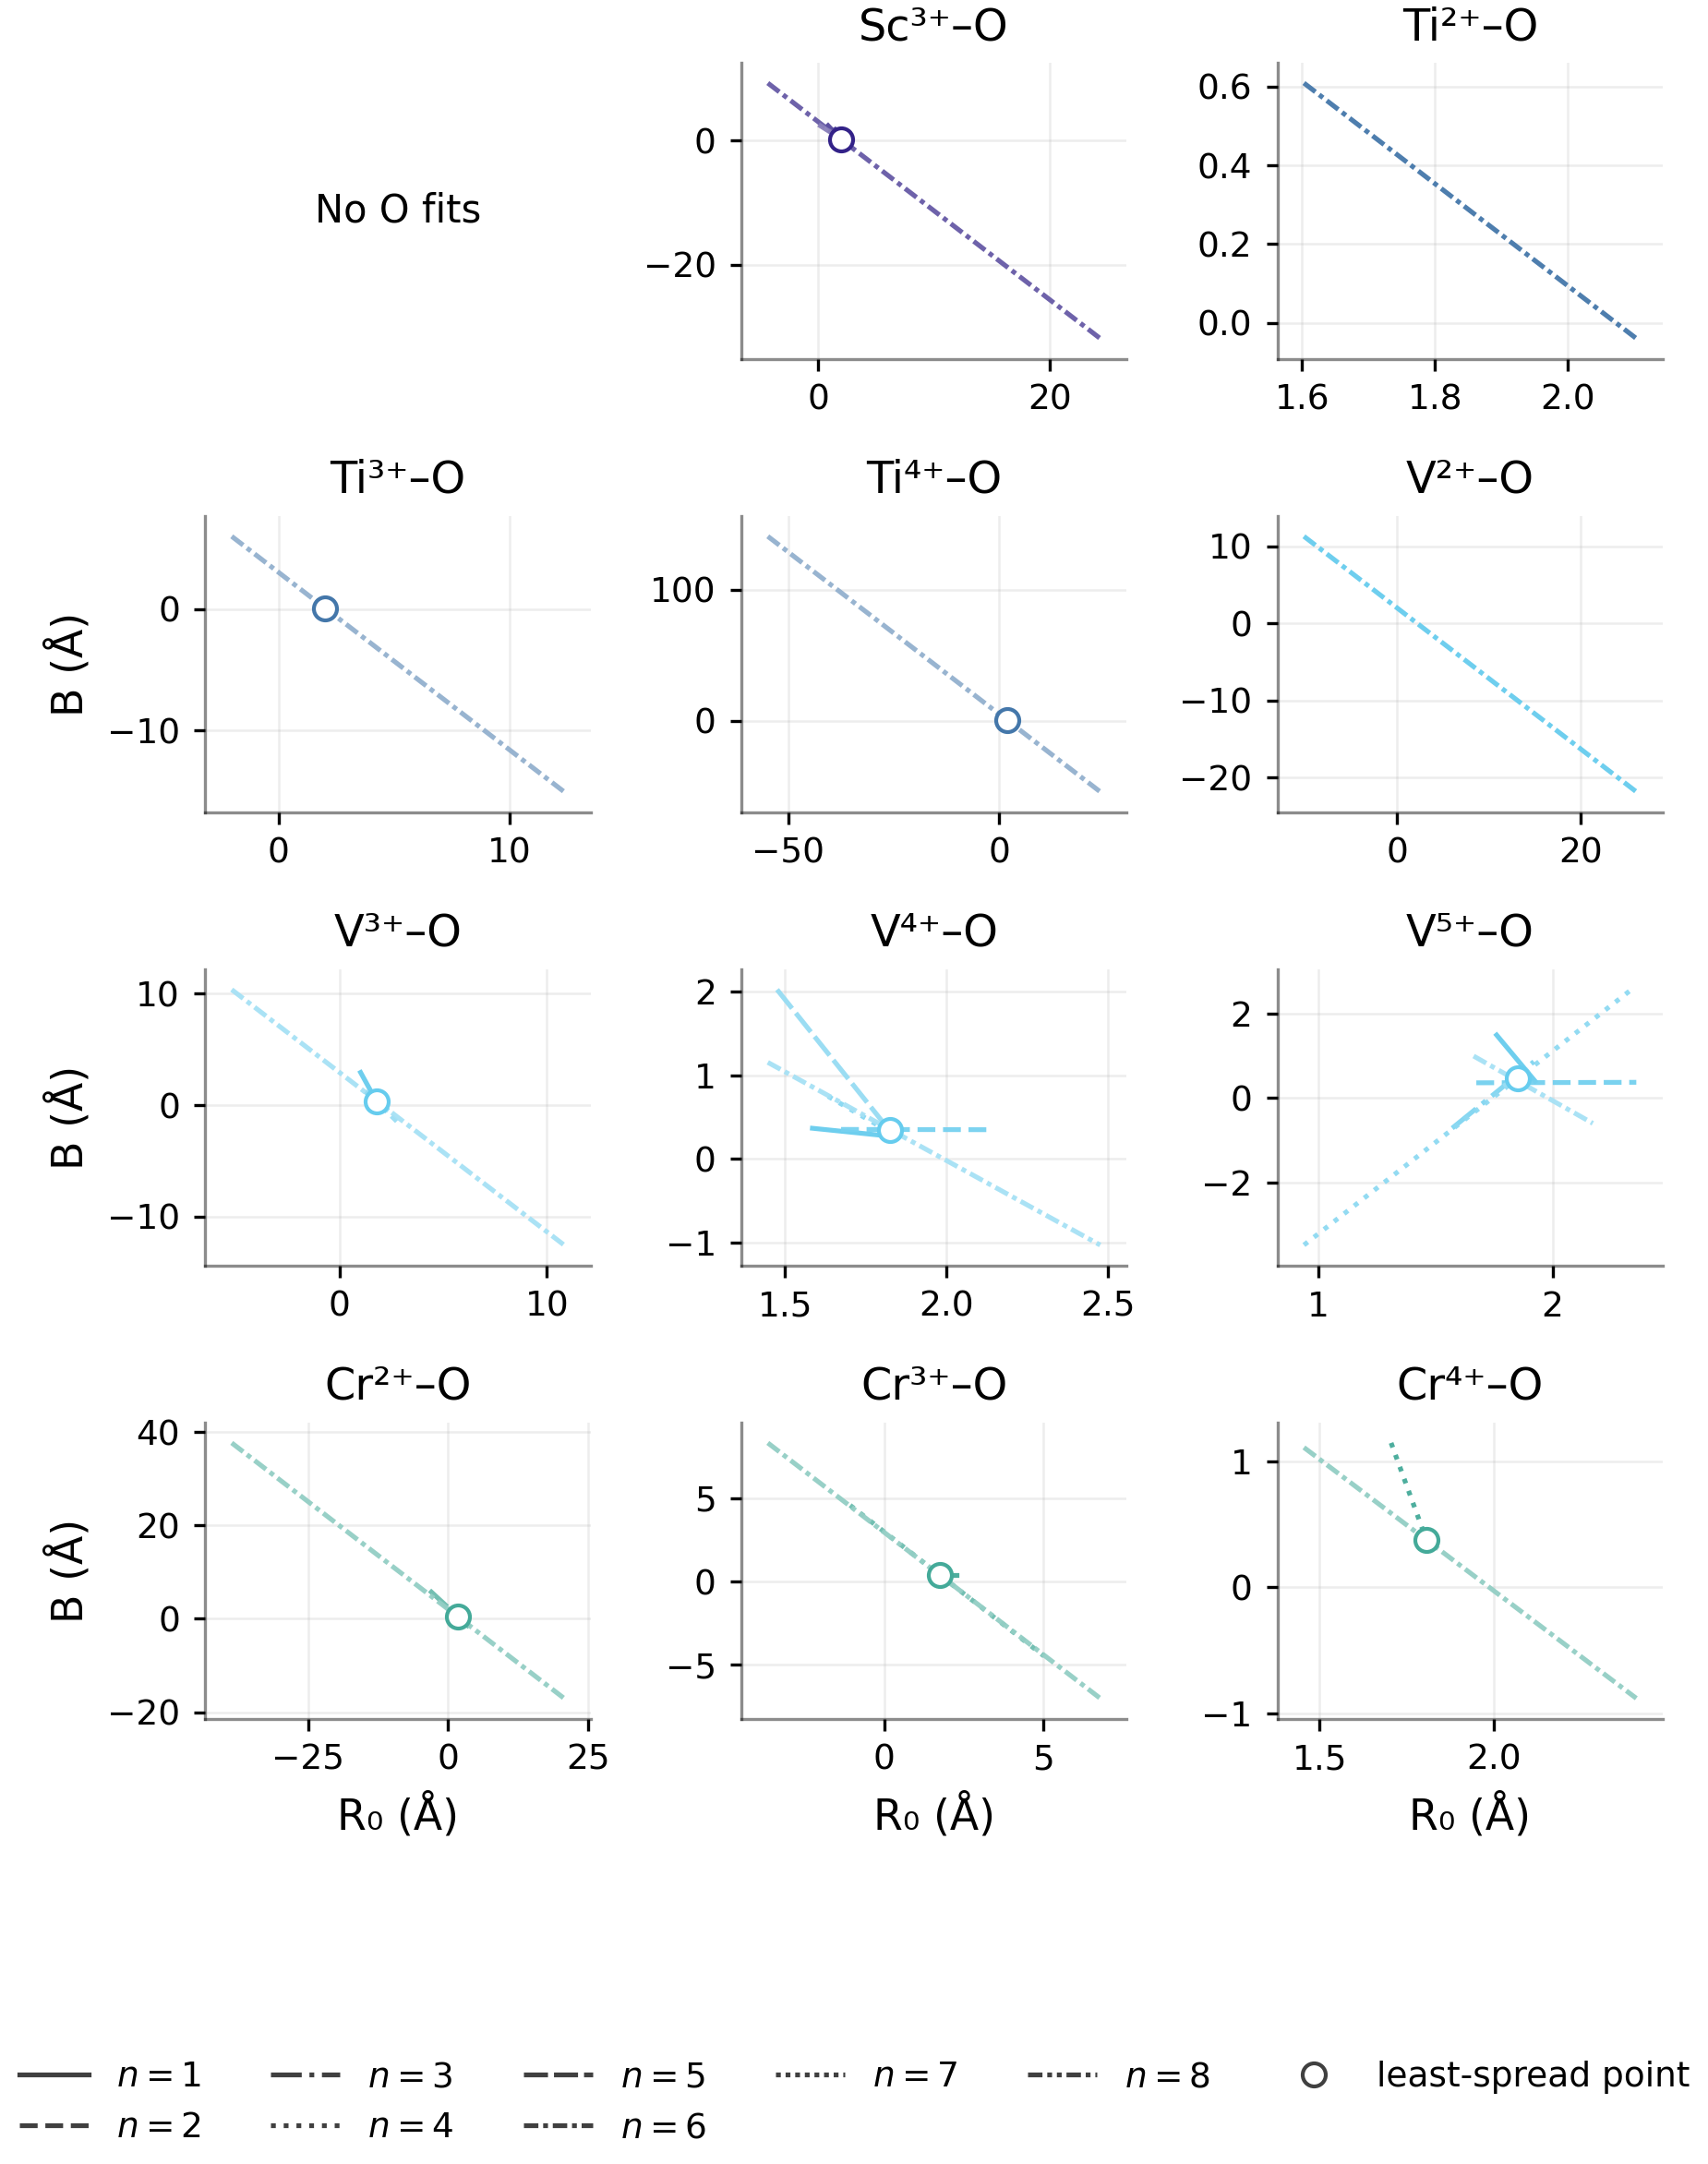
\includegraphics[width=\textwidth]{dblock_oxi_oxygen_cn_fit_lines_part01.png}
\caption{$n$-resolved $B$ vs.\ $R_0$ for oxidation-state--resolved 3$d$
X--O pairs (Sc--Cr).}
\label{fig:dblock_fits_1}
\end{figure}

\begin{figure}[p]
\centering
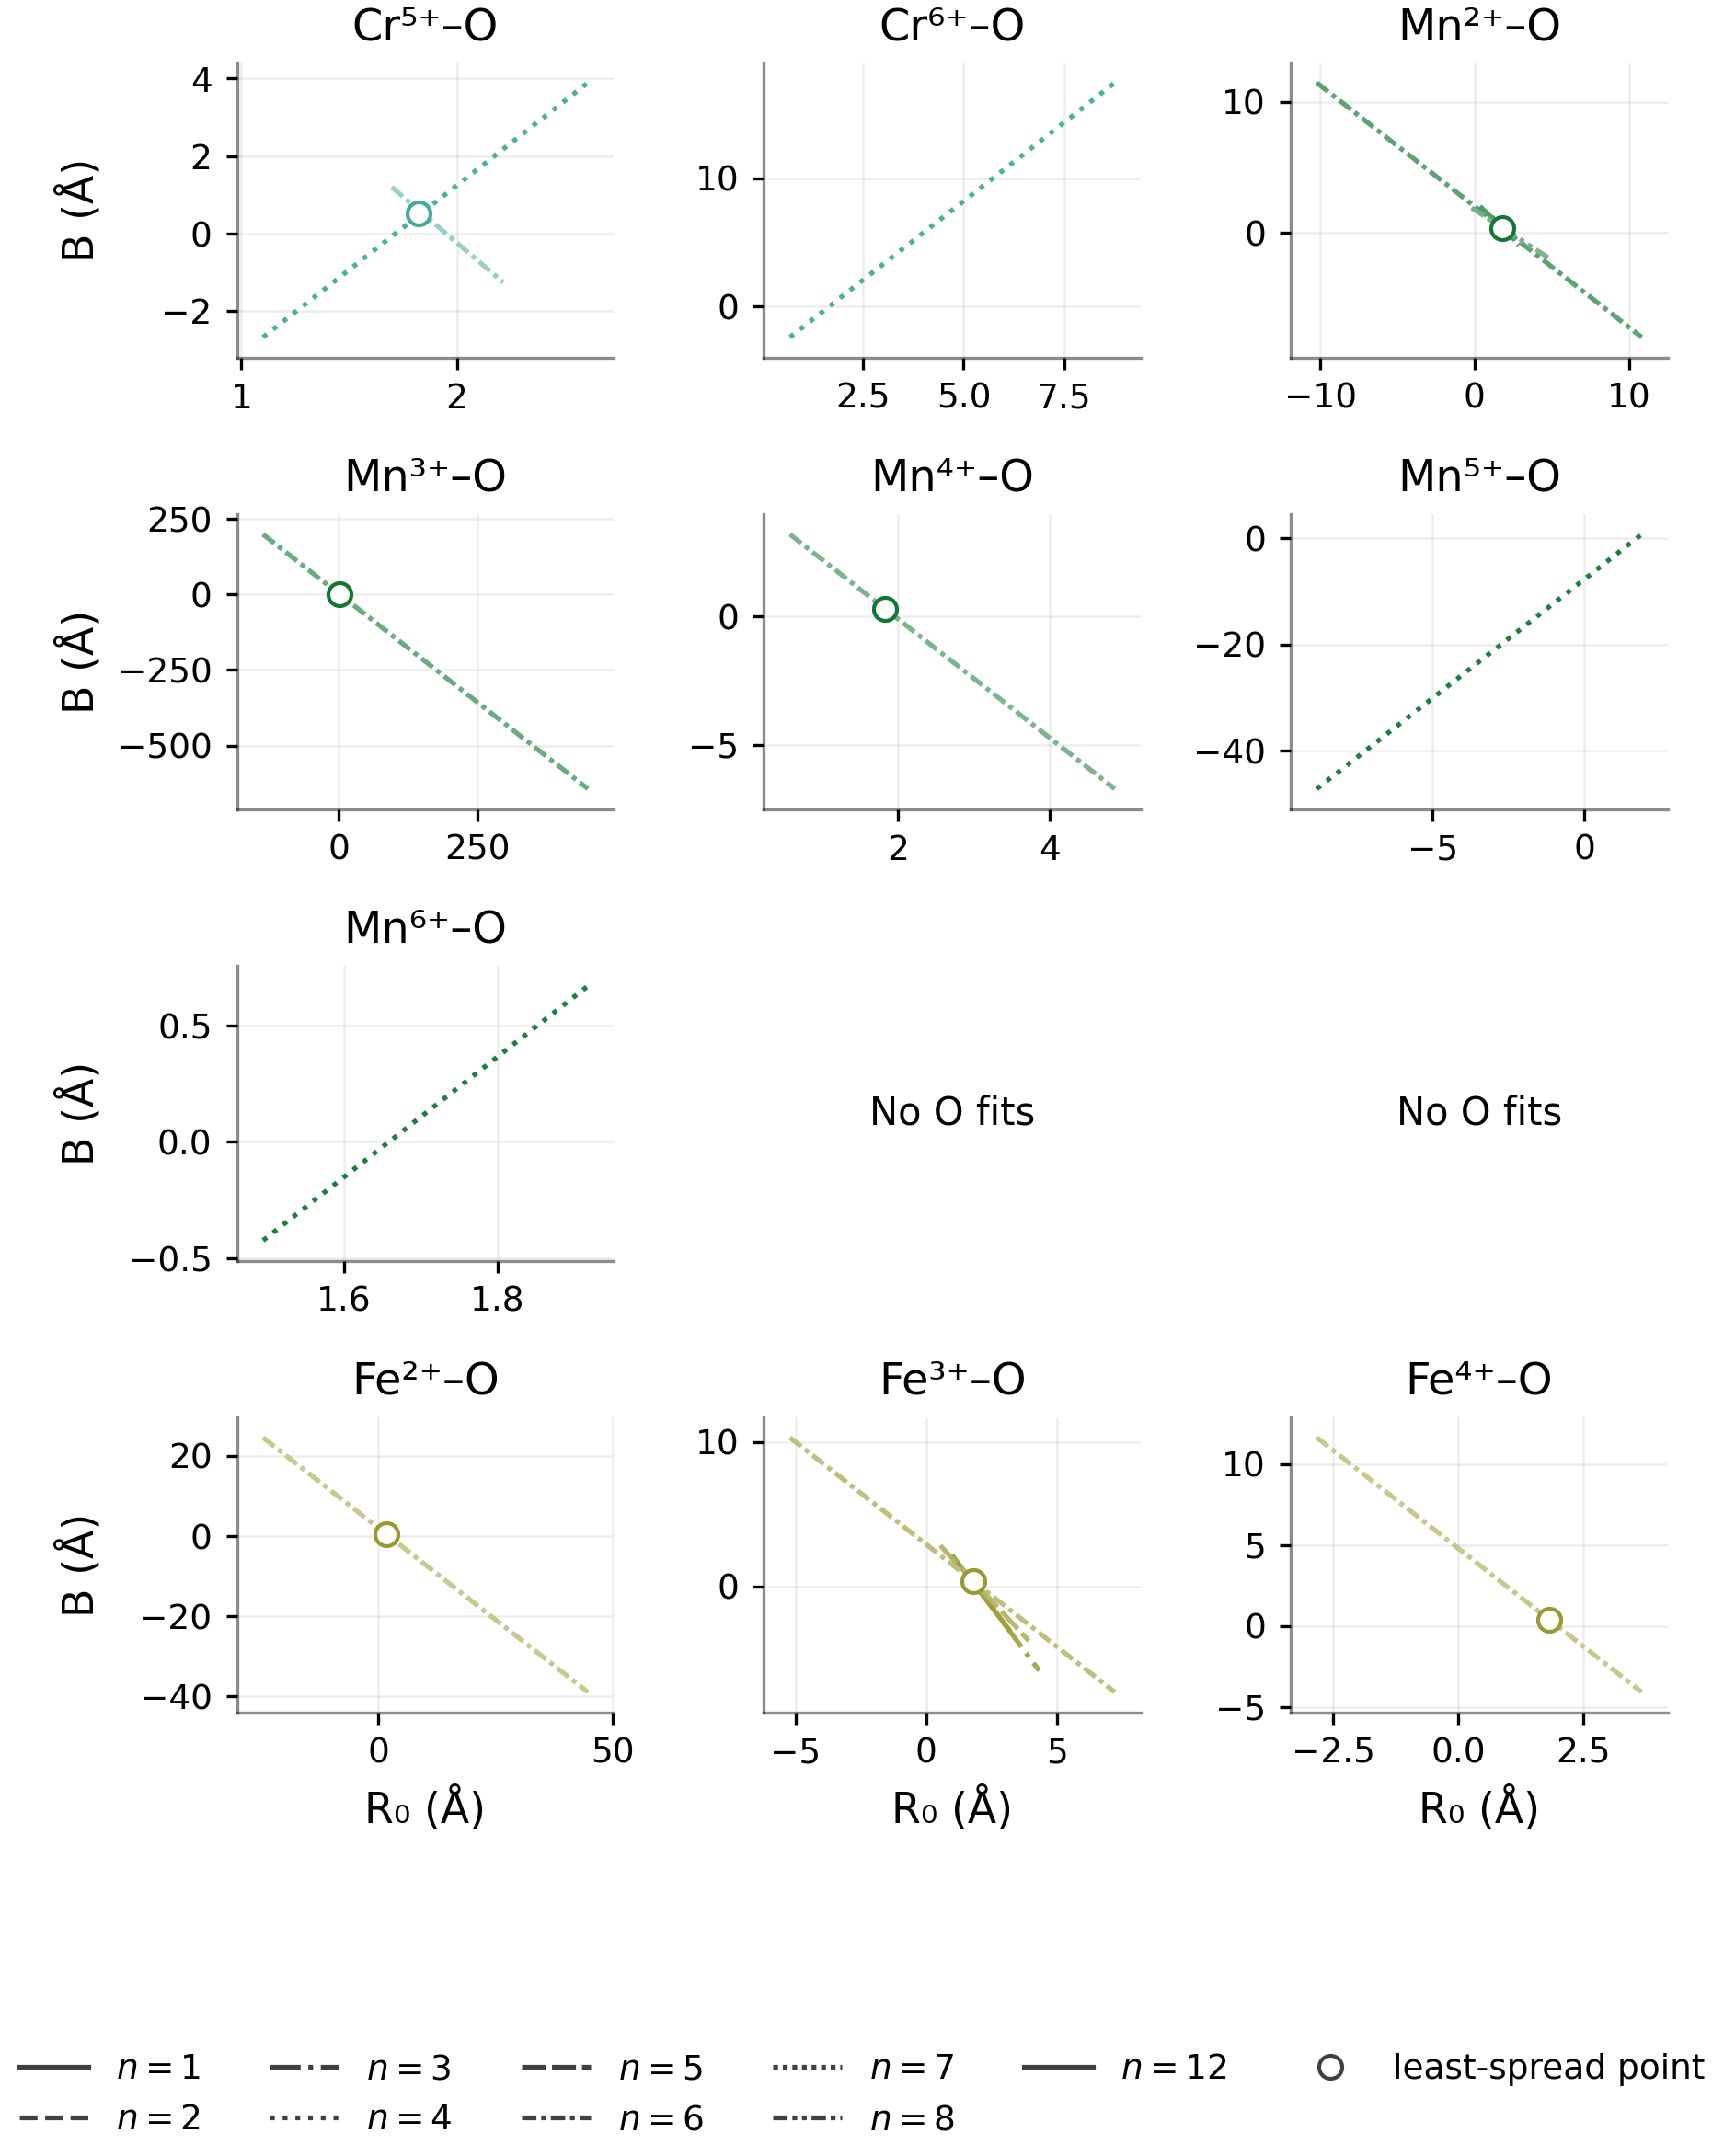
\includegraphics[width=\textwidth]{dblock_oxi_oxygen_cn_fit_lines_part02.png}
\caption{$n$-resolved $B$ vs.\ $R_0$ for oxidation-state--resolved 3$d$
X--O pairs (Cr$^{5+}$--Fe$^{4+}$).}
\label{fig:dblock_fits_2}
\end{figure}

\begin{figure}[p]
\centering
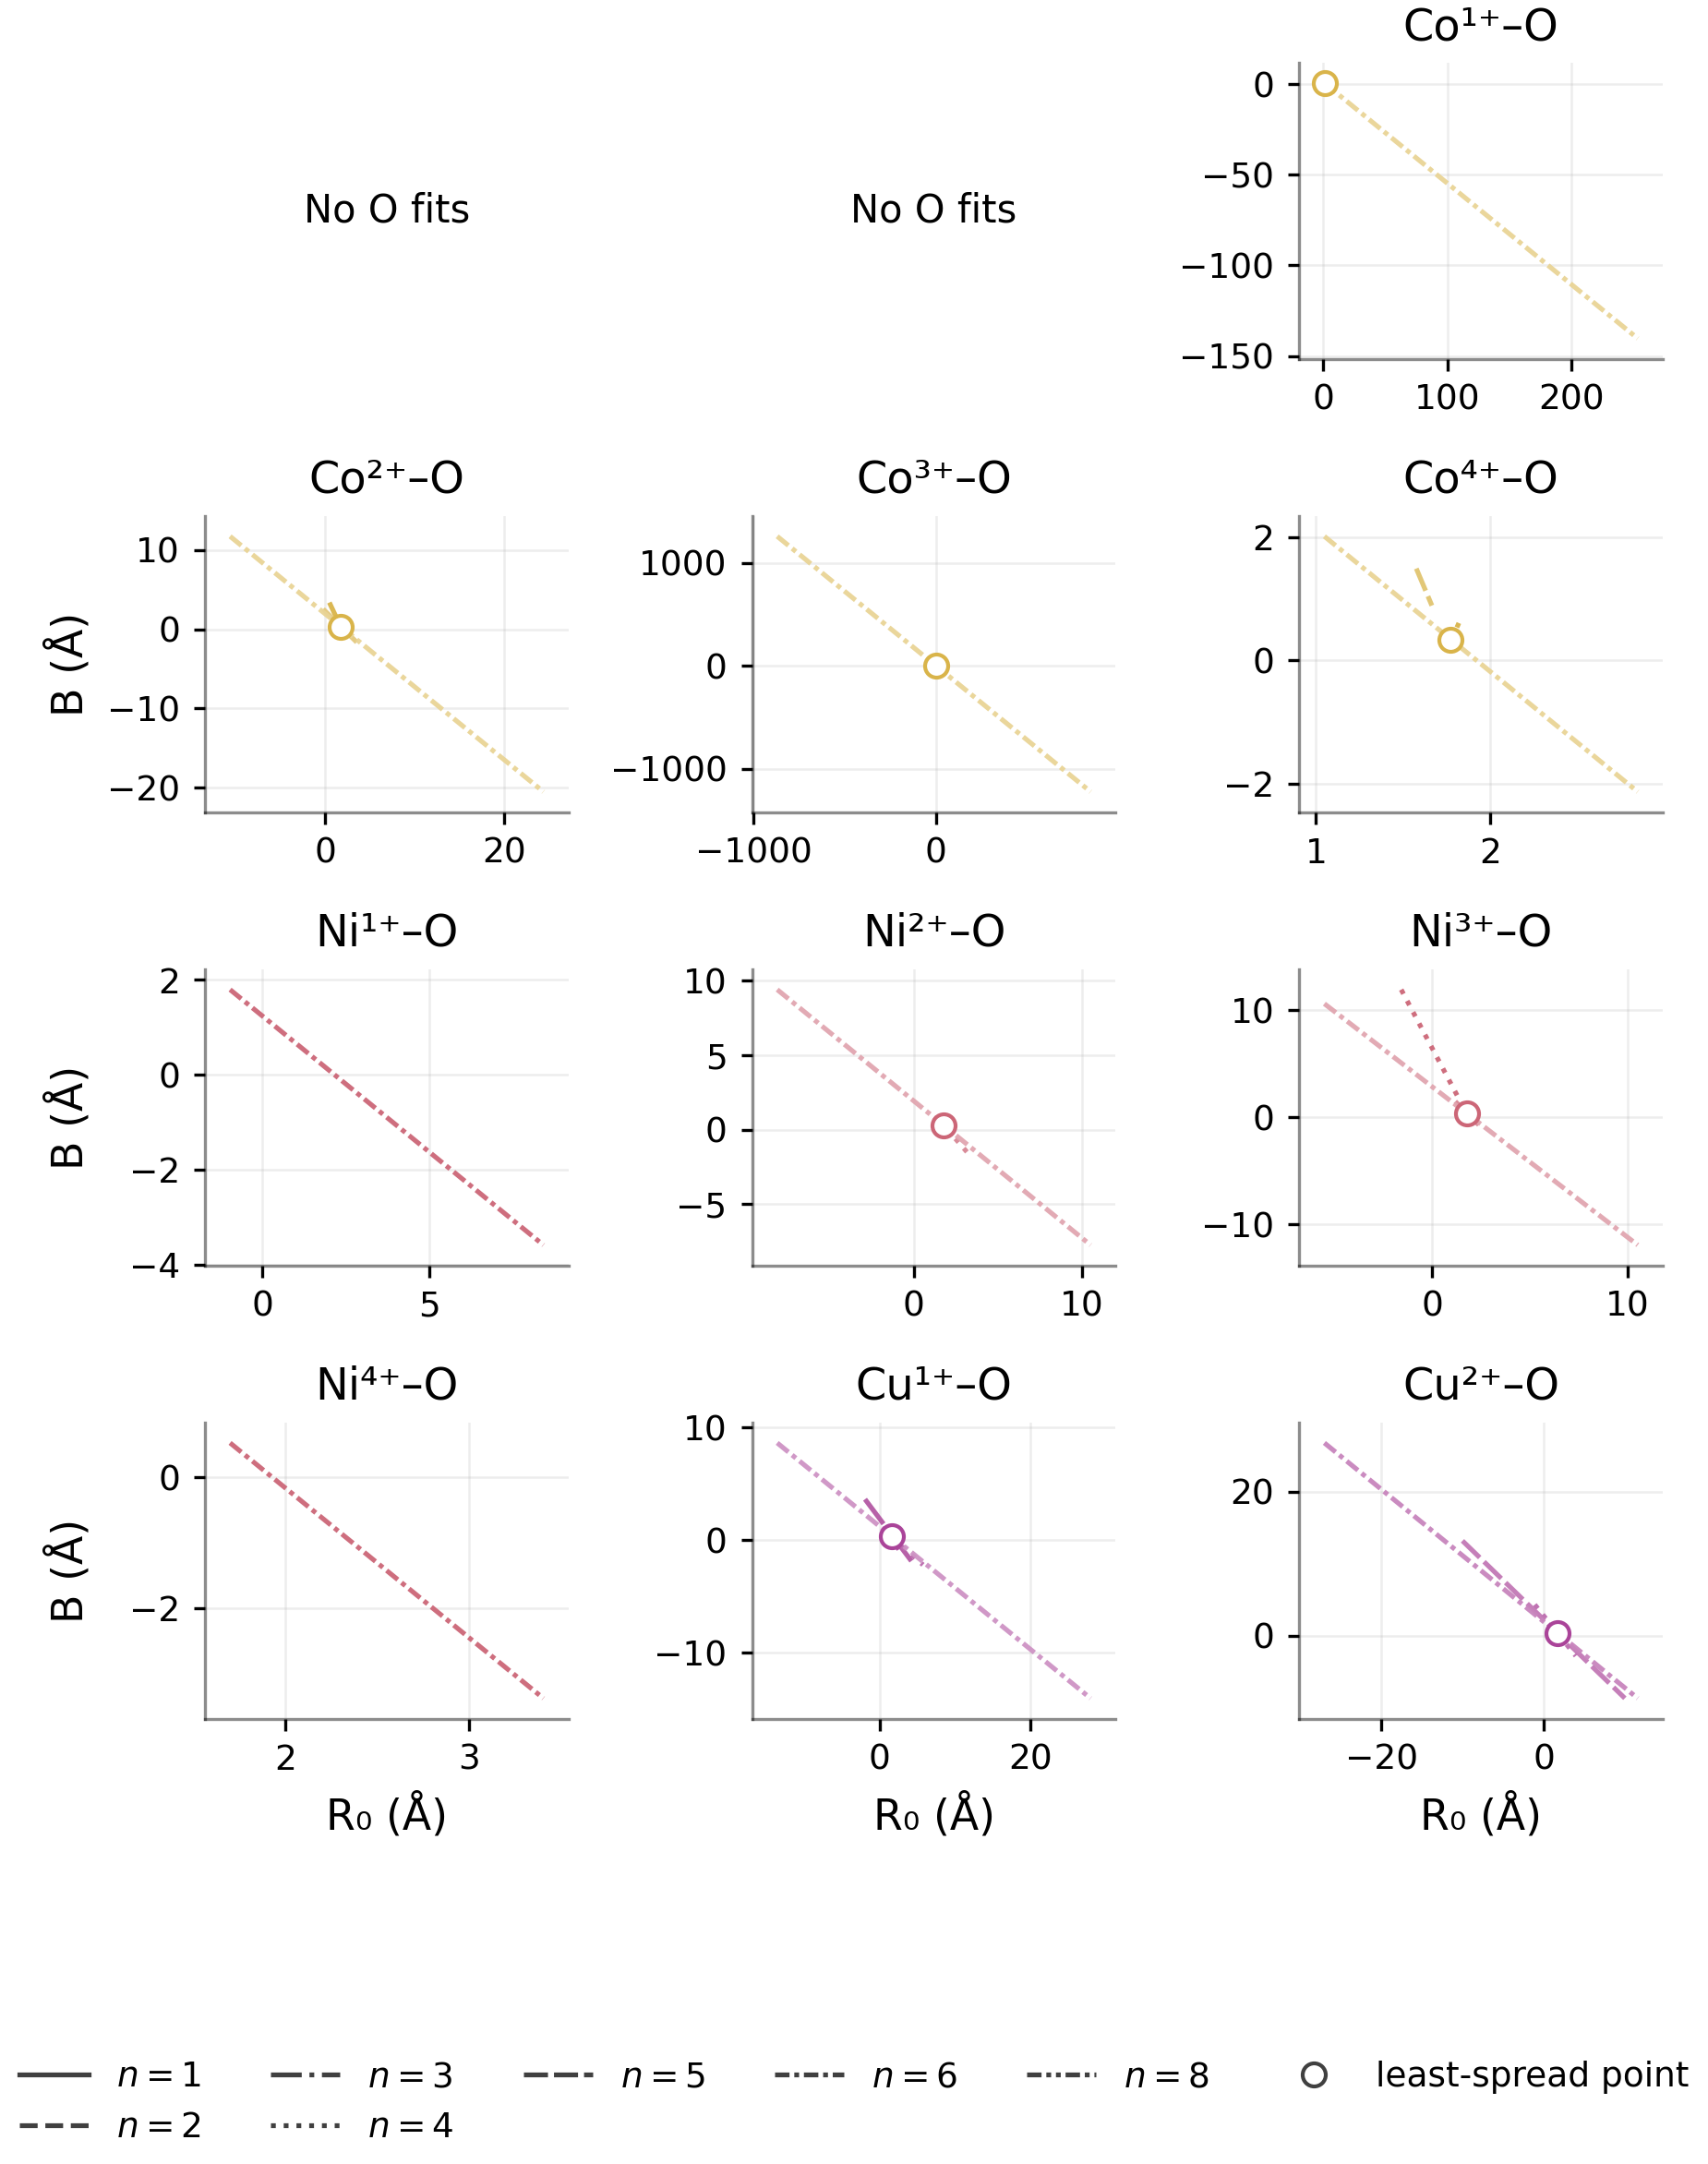
\includegraphics[width=\textwidth]{dblock_oxi_oxygen_cn_fit_lines_part03.png}
\caption{$n$-resolved $B$ vs.\ $R_0$ for oxidation-state--resolved 3$d$
X--O pairs (Co--Cu$^{2+}$).}
\label{fig:dblock_fits_3}
\end{figure}

\begin{figure}[p]
\centering
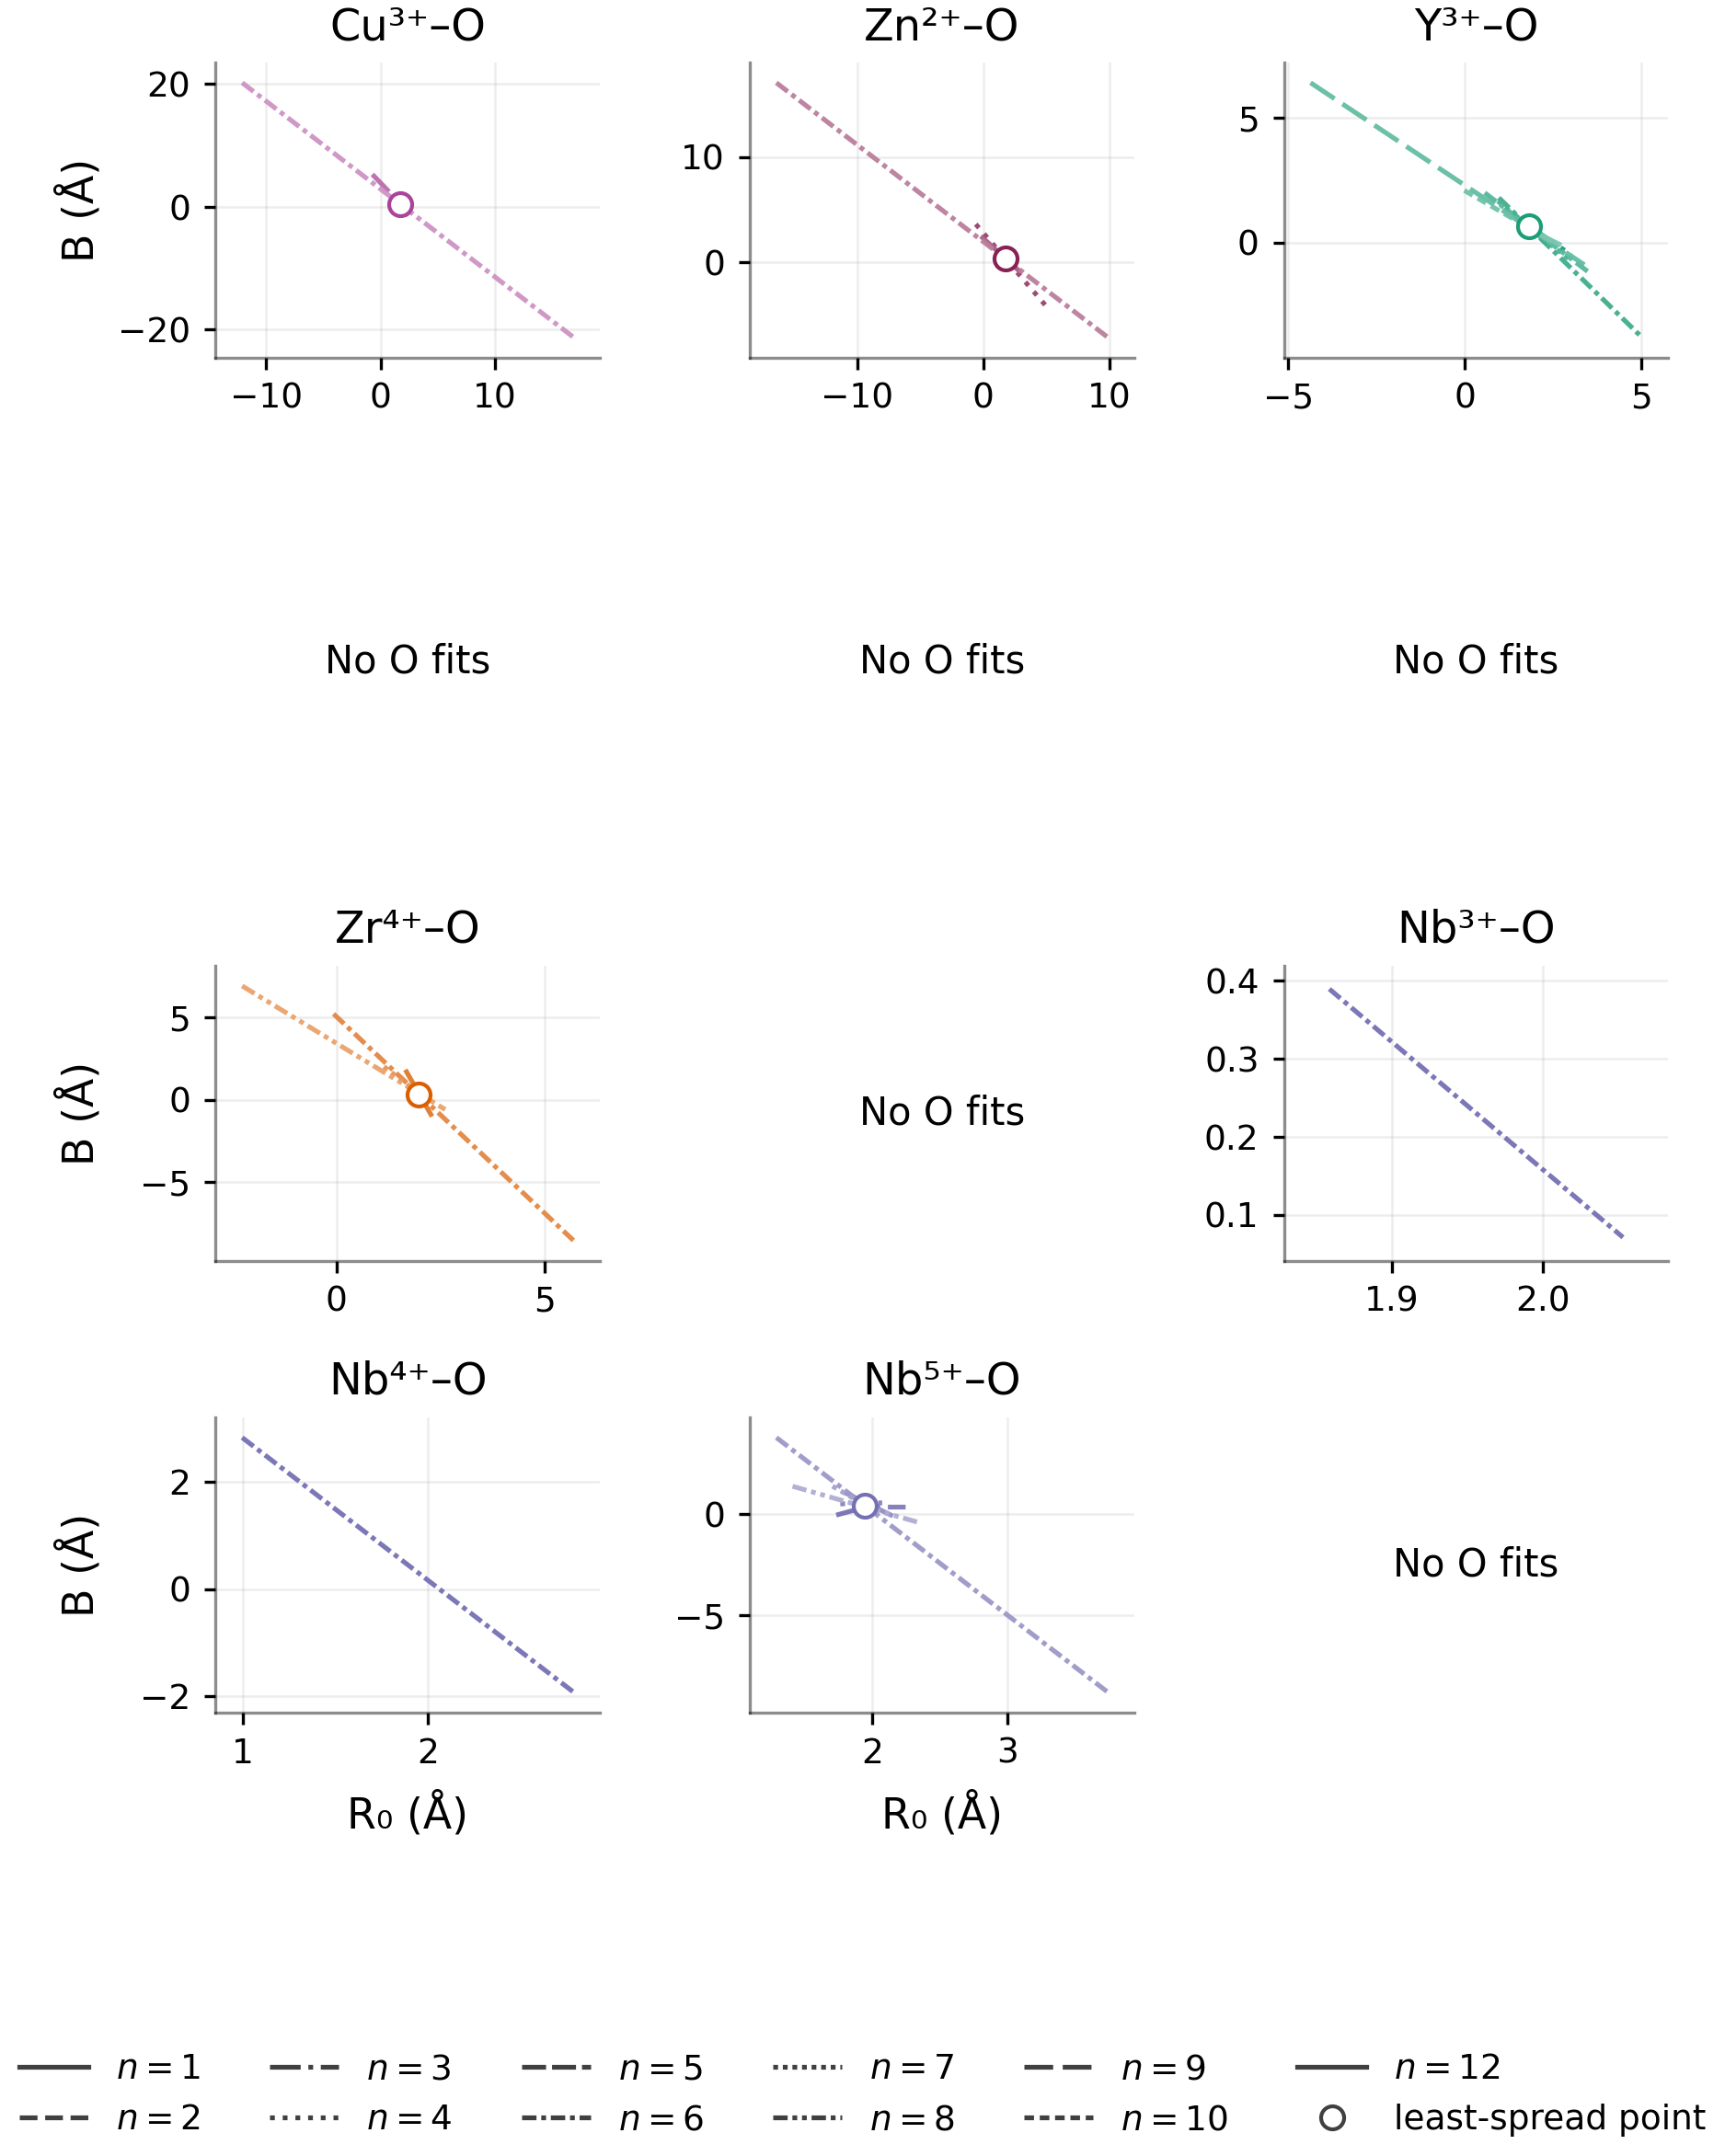
\includegraphics[width=\textwidth]{dblock_oxi_oxygen_cn_fit_lines_part04.png}
\caption{$n$-resolved $B$ vs.\ $R_0$ for oxidation-state--resolved 3$d$/4$d$
X--O pairs (Cu$^{3+}$--Nb).}
\label{fig:dblock_fits_4}
\end{figure}

\begin{figure}[p]
\centering
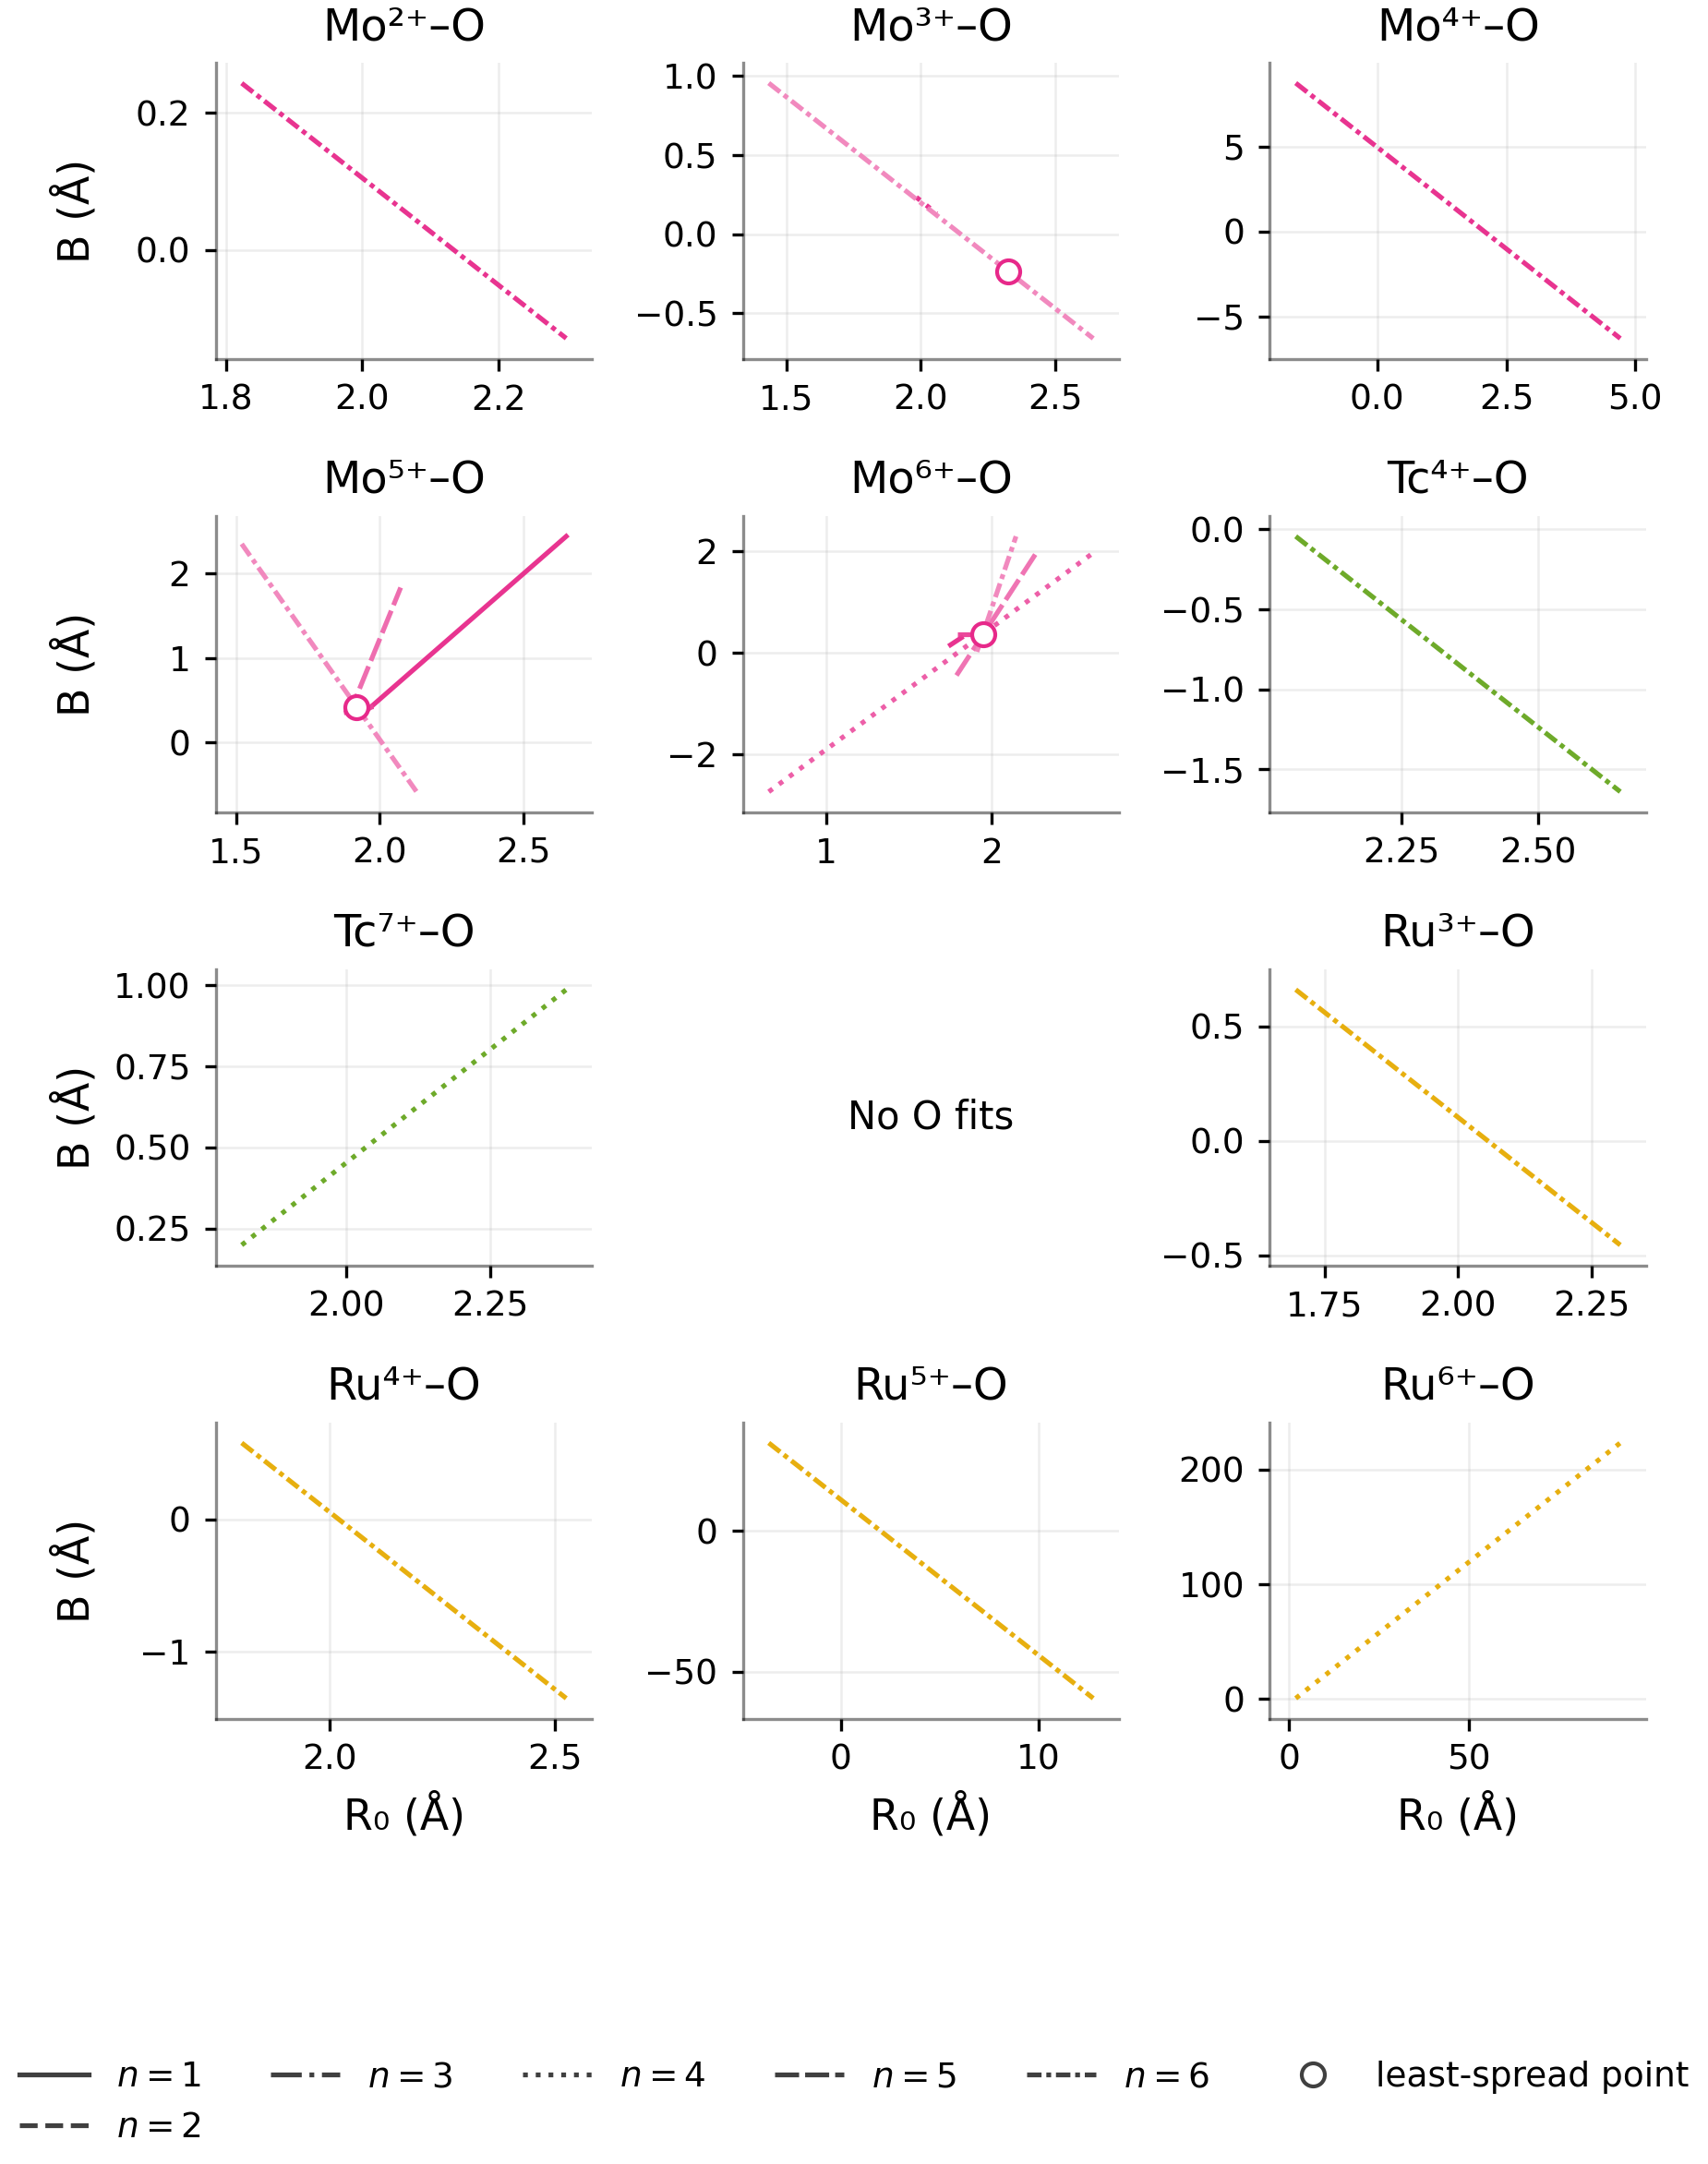
\includegraphics[width=\textwidth]{dblock_oxi_oxygen_cn_fit_lines_part05.png}
\caption{$n$-resolved $B$ vs.\ $R_0$ for oxidation-state--resolved 4$d$
X--O pairs (Mo--Ru).}
\label{fig:dblock_fits_5}
\end{figure}

\begin{figure}[p]
\centering
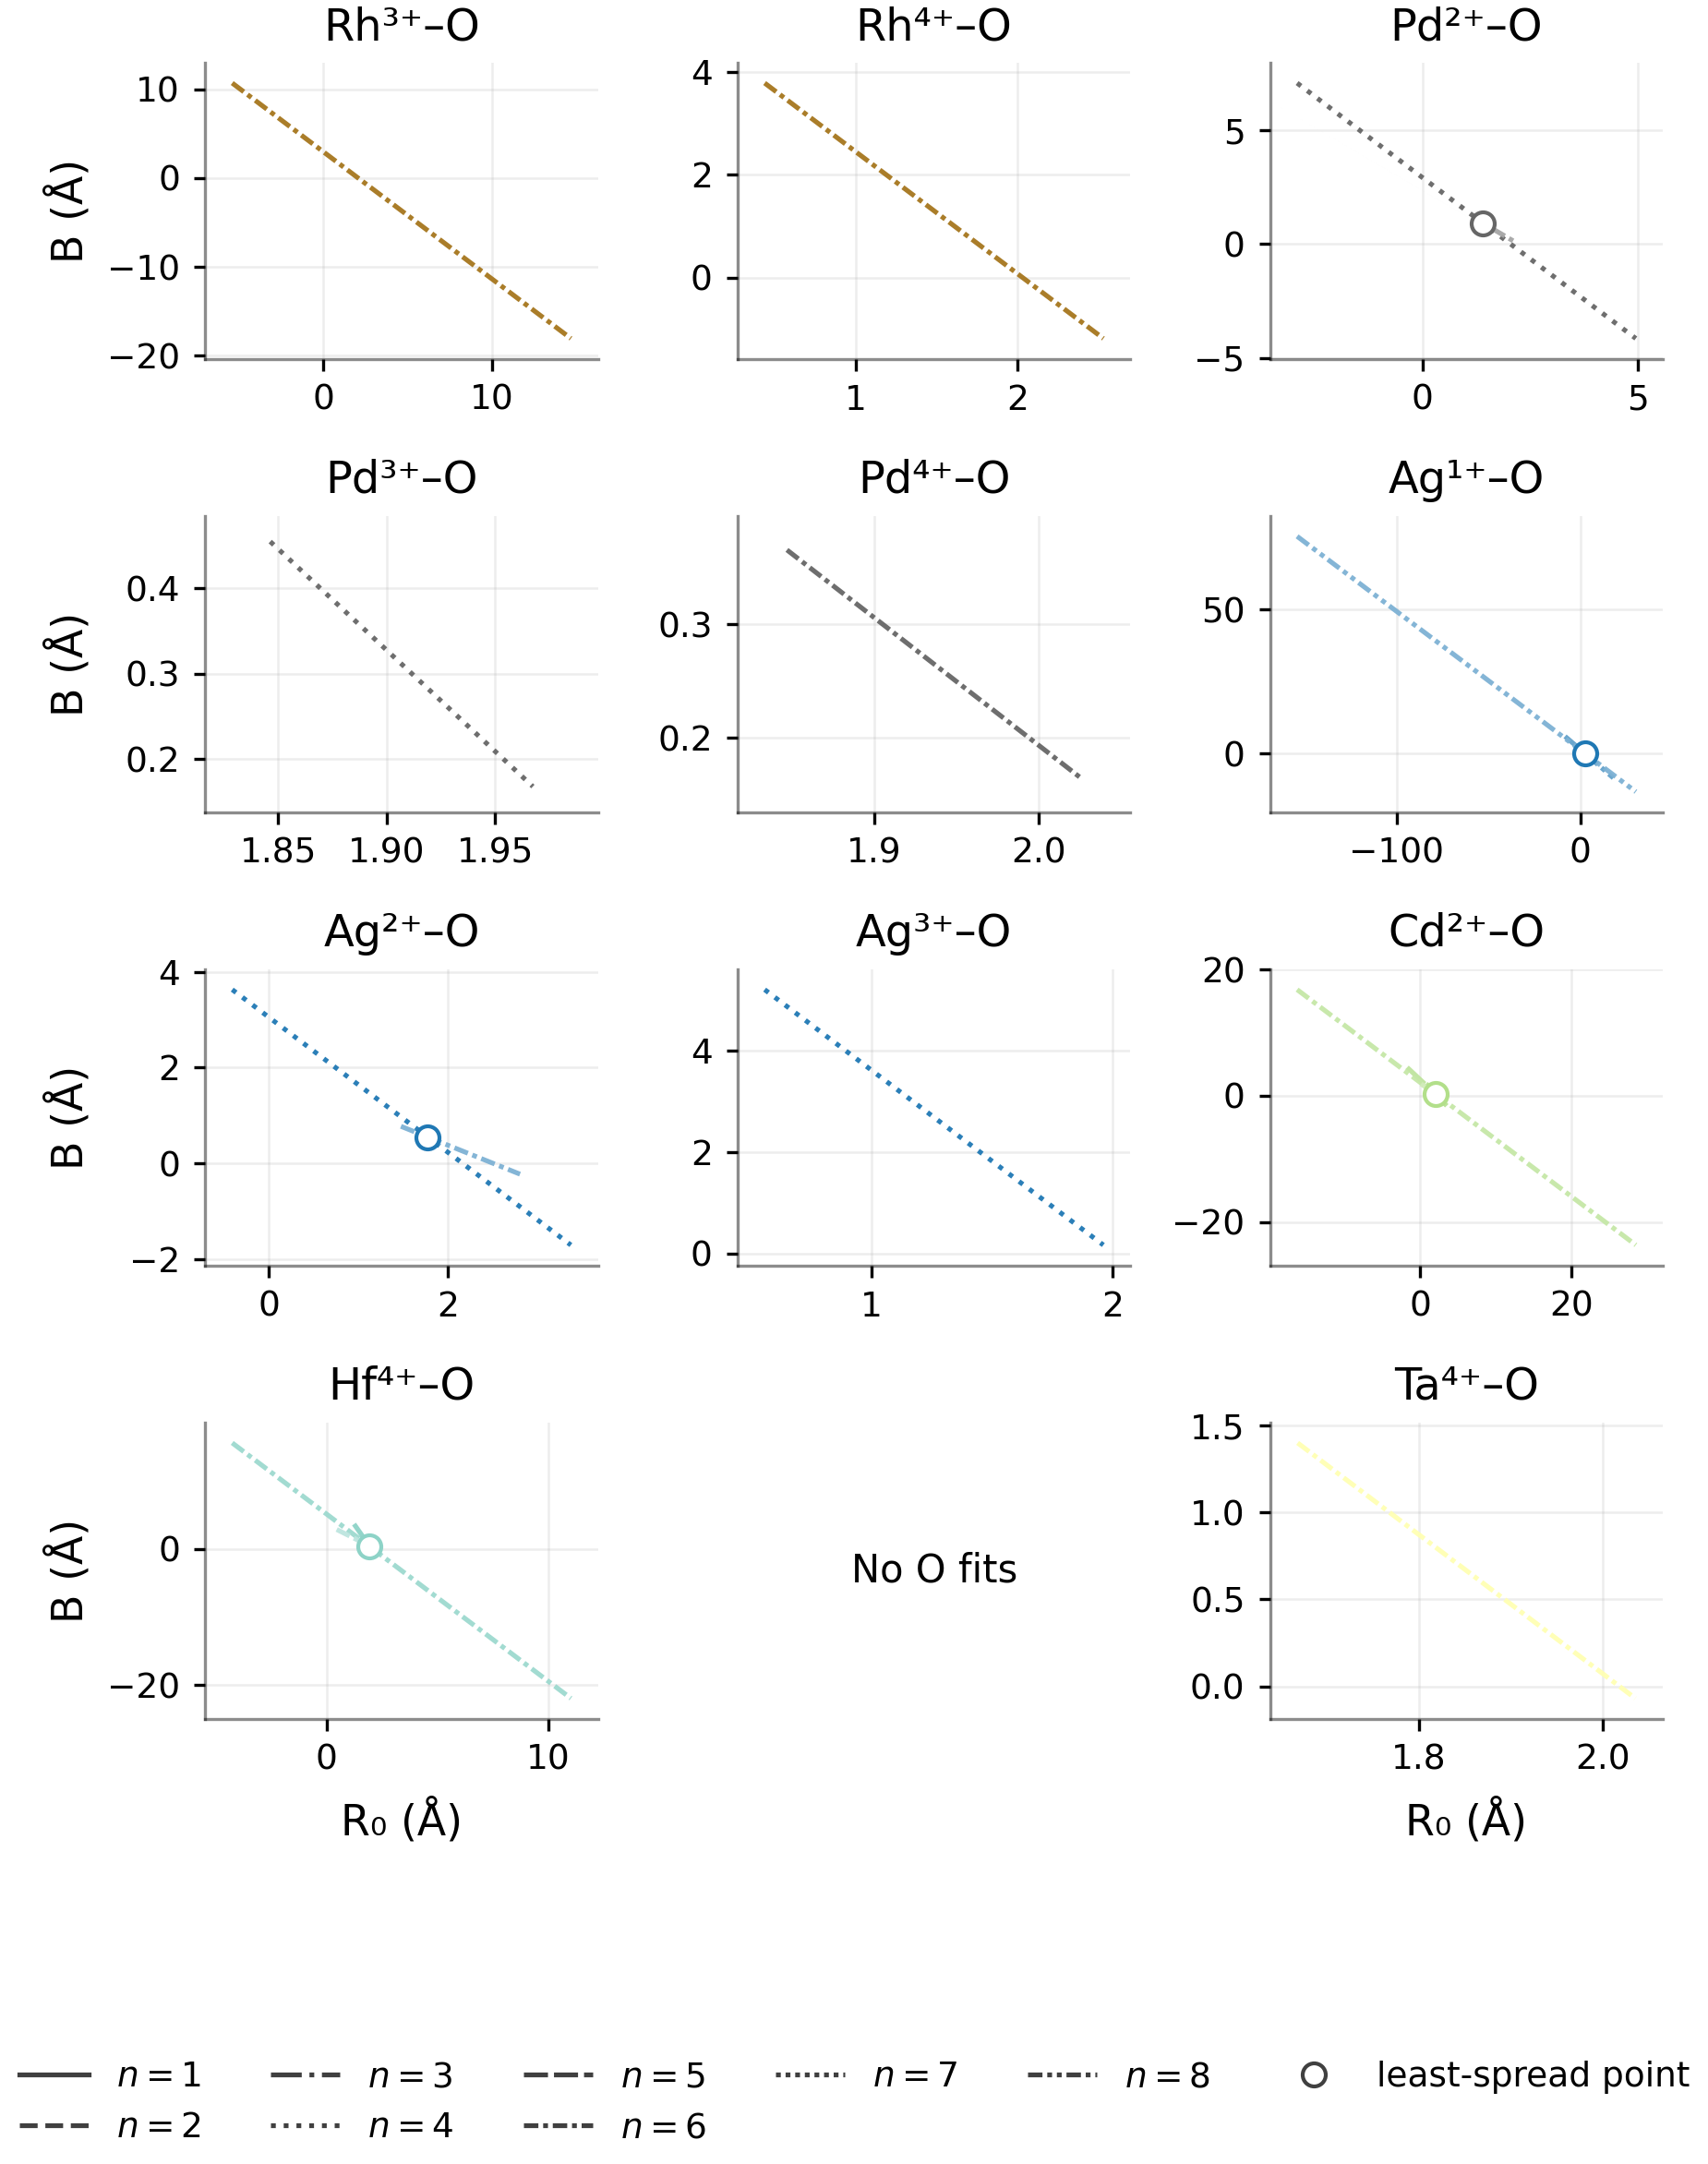
\includegraphics[width=\textwidth]{dblock_oxi_oxygen_cn_fit_lines_part06.png}
\caption{$n$-resolved $B$ vs.\ $R_0$ for oxidation-state--resolved 4$d$/5$d$
X--O pairs (Rh--Ta$^{4+}$).}
\label{fig:dblock_fits_6}
\end{figure}

\begin{figure}[p]
\centering
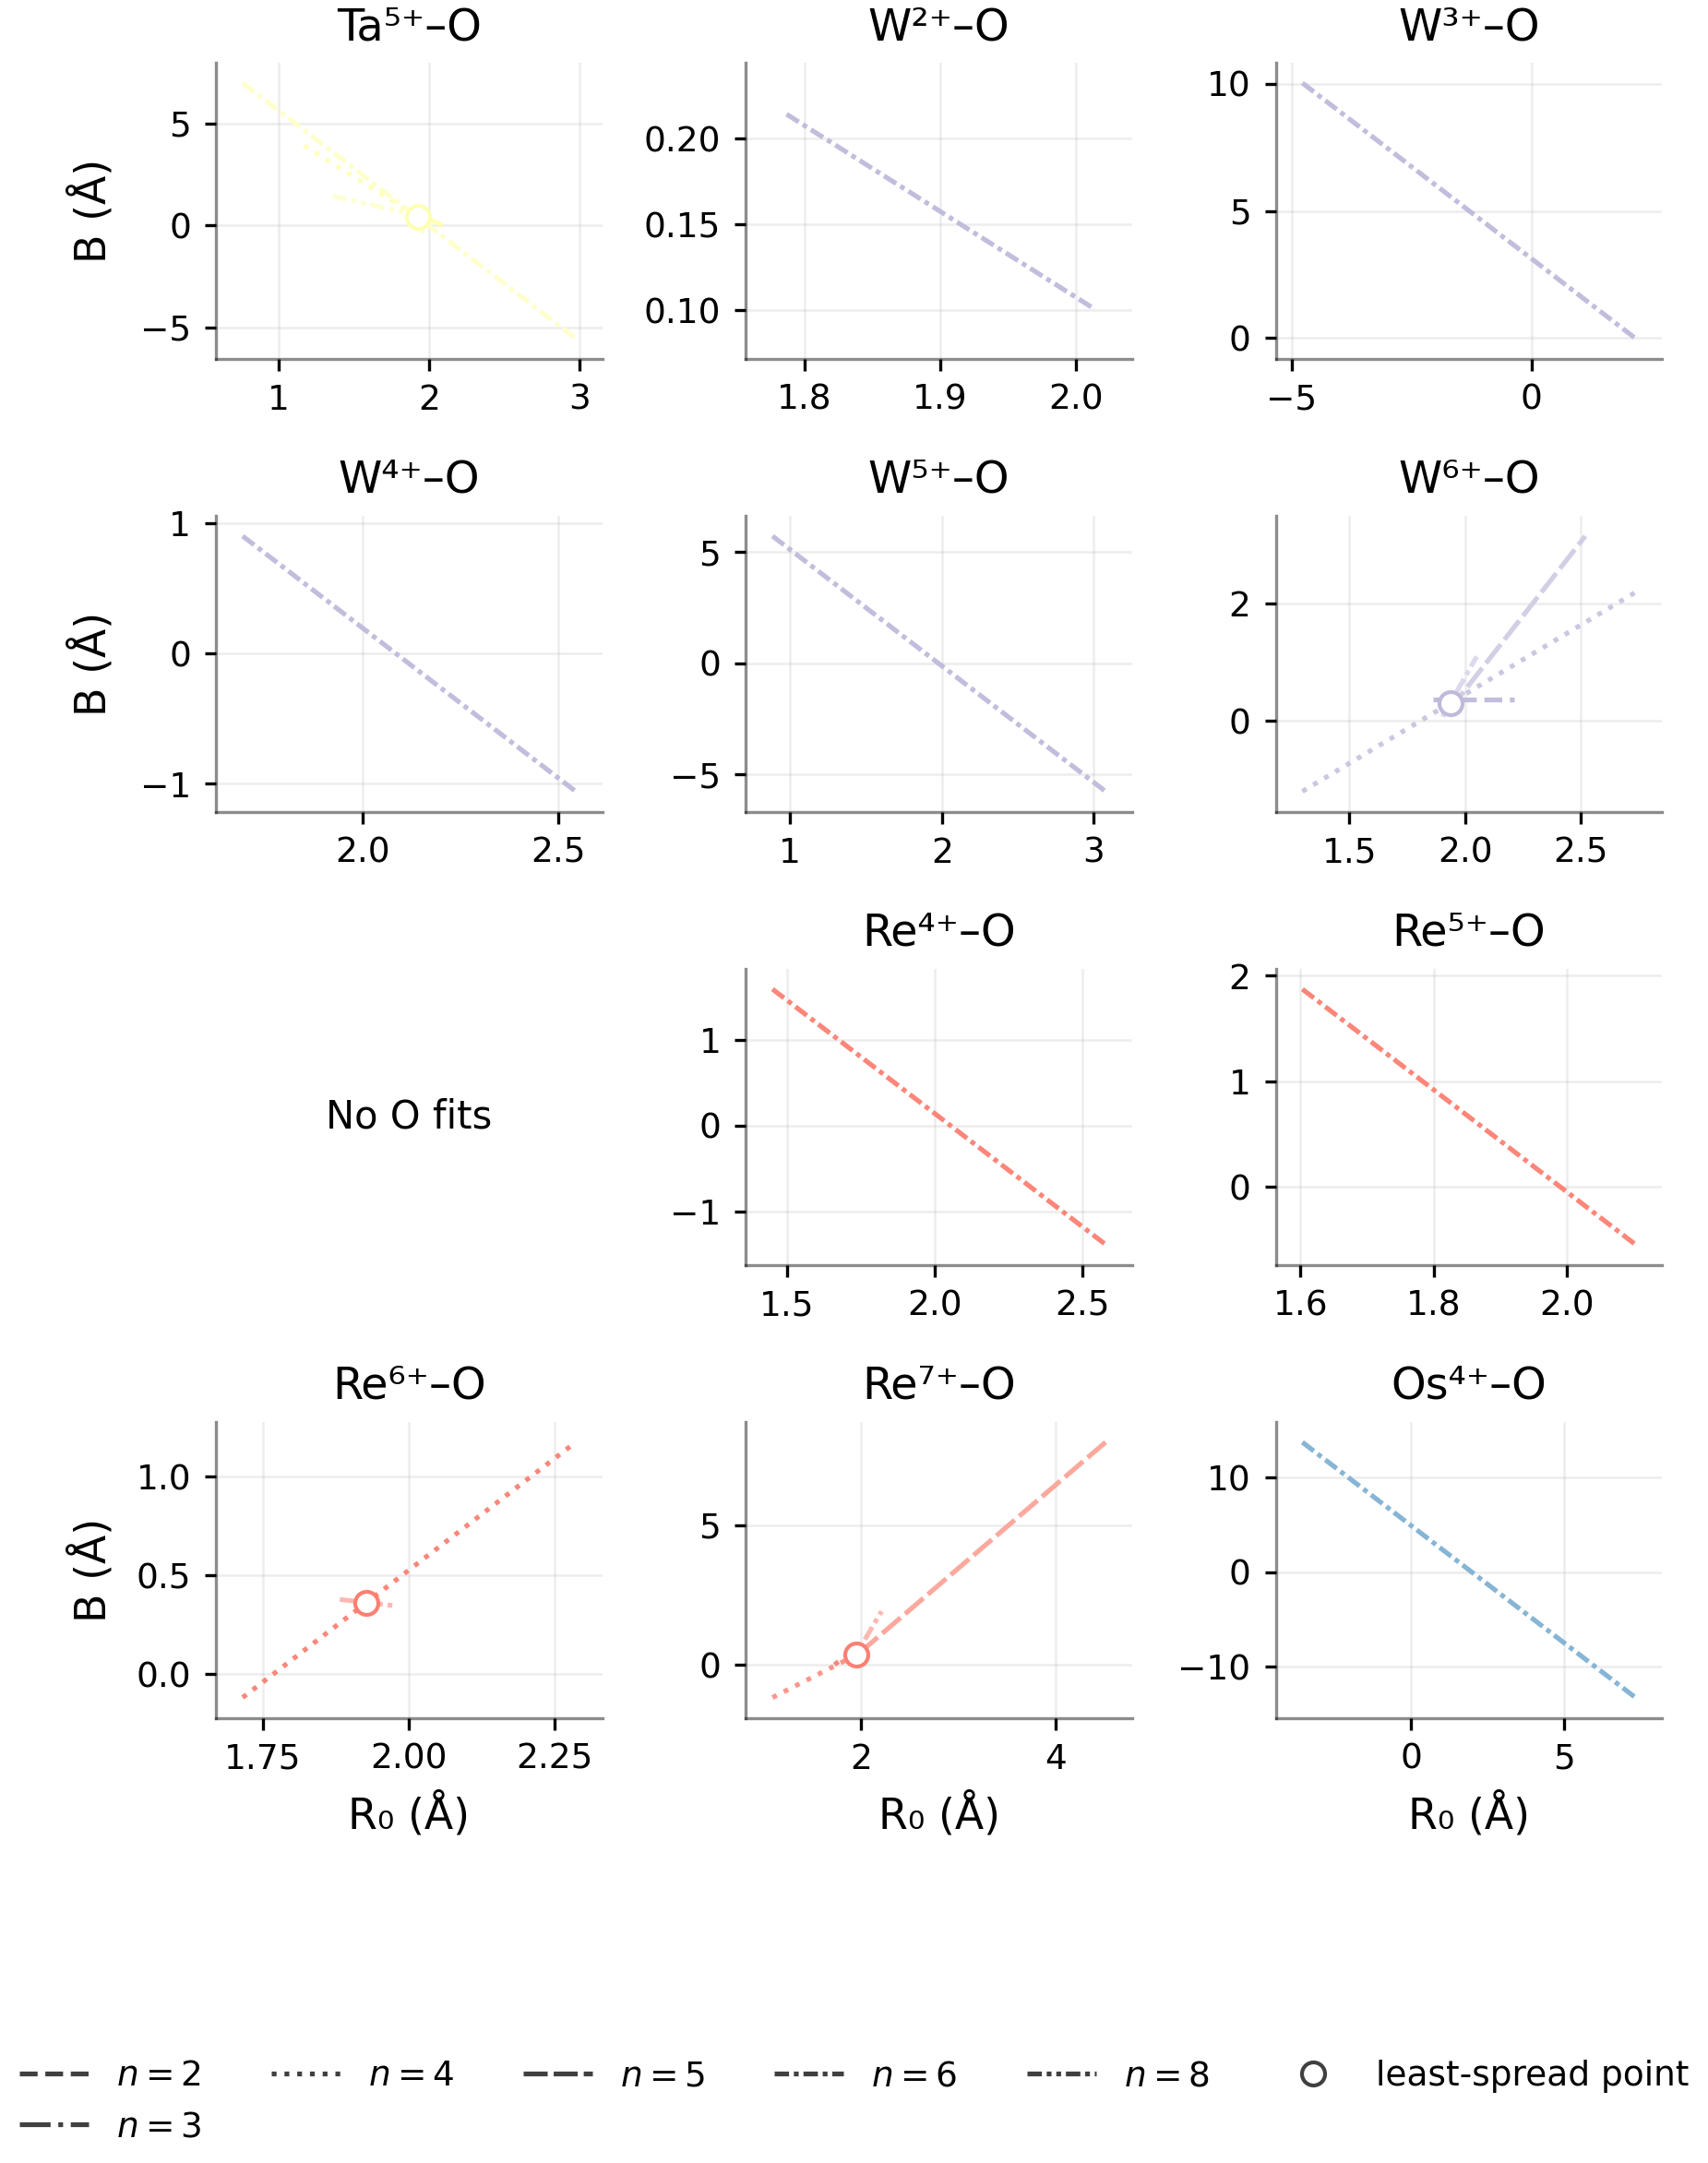
\includegraphics[width=\textwidth]{dblock_oxi_oxygen_cn_fit_lines_part07.png}
\caption{$n$-resolved $B$ vs.\ $R_0$ for oxidation-state--resolved 5$d$
X--O pairs (Ta$^{5+}$--Os).}
\label{fig:dblock_fits_7}
\end{figure}

\begin{figure}[p]
\centering
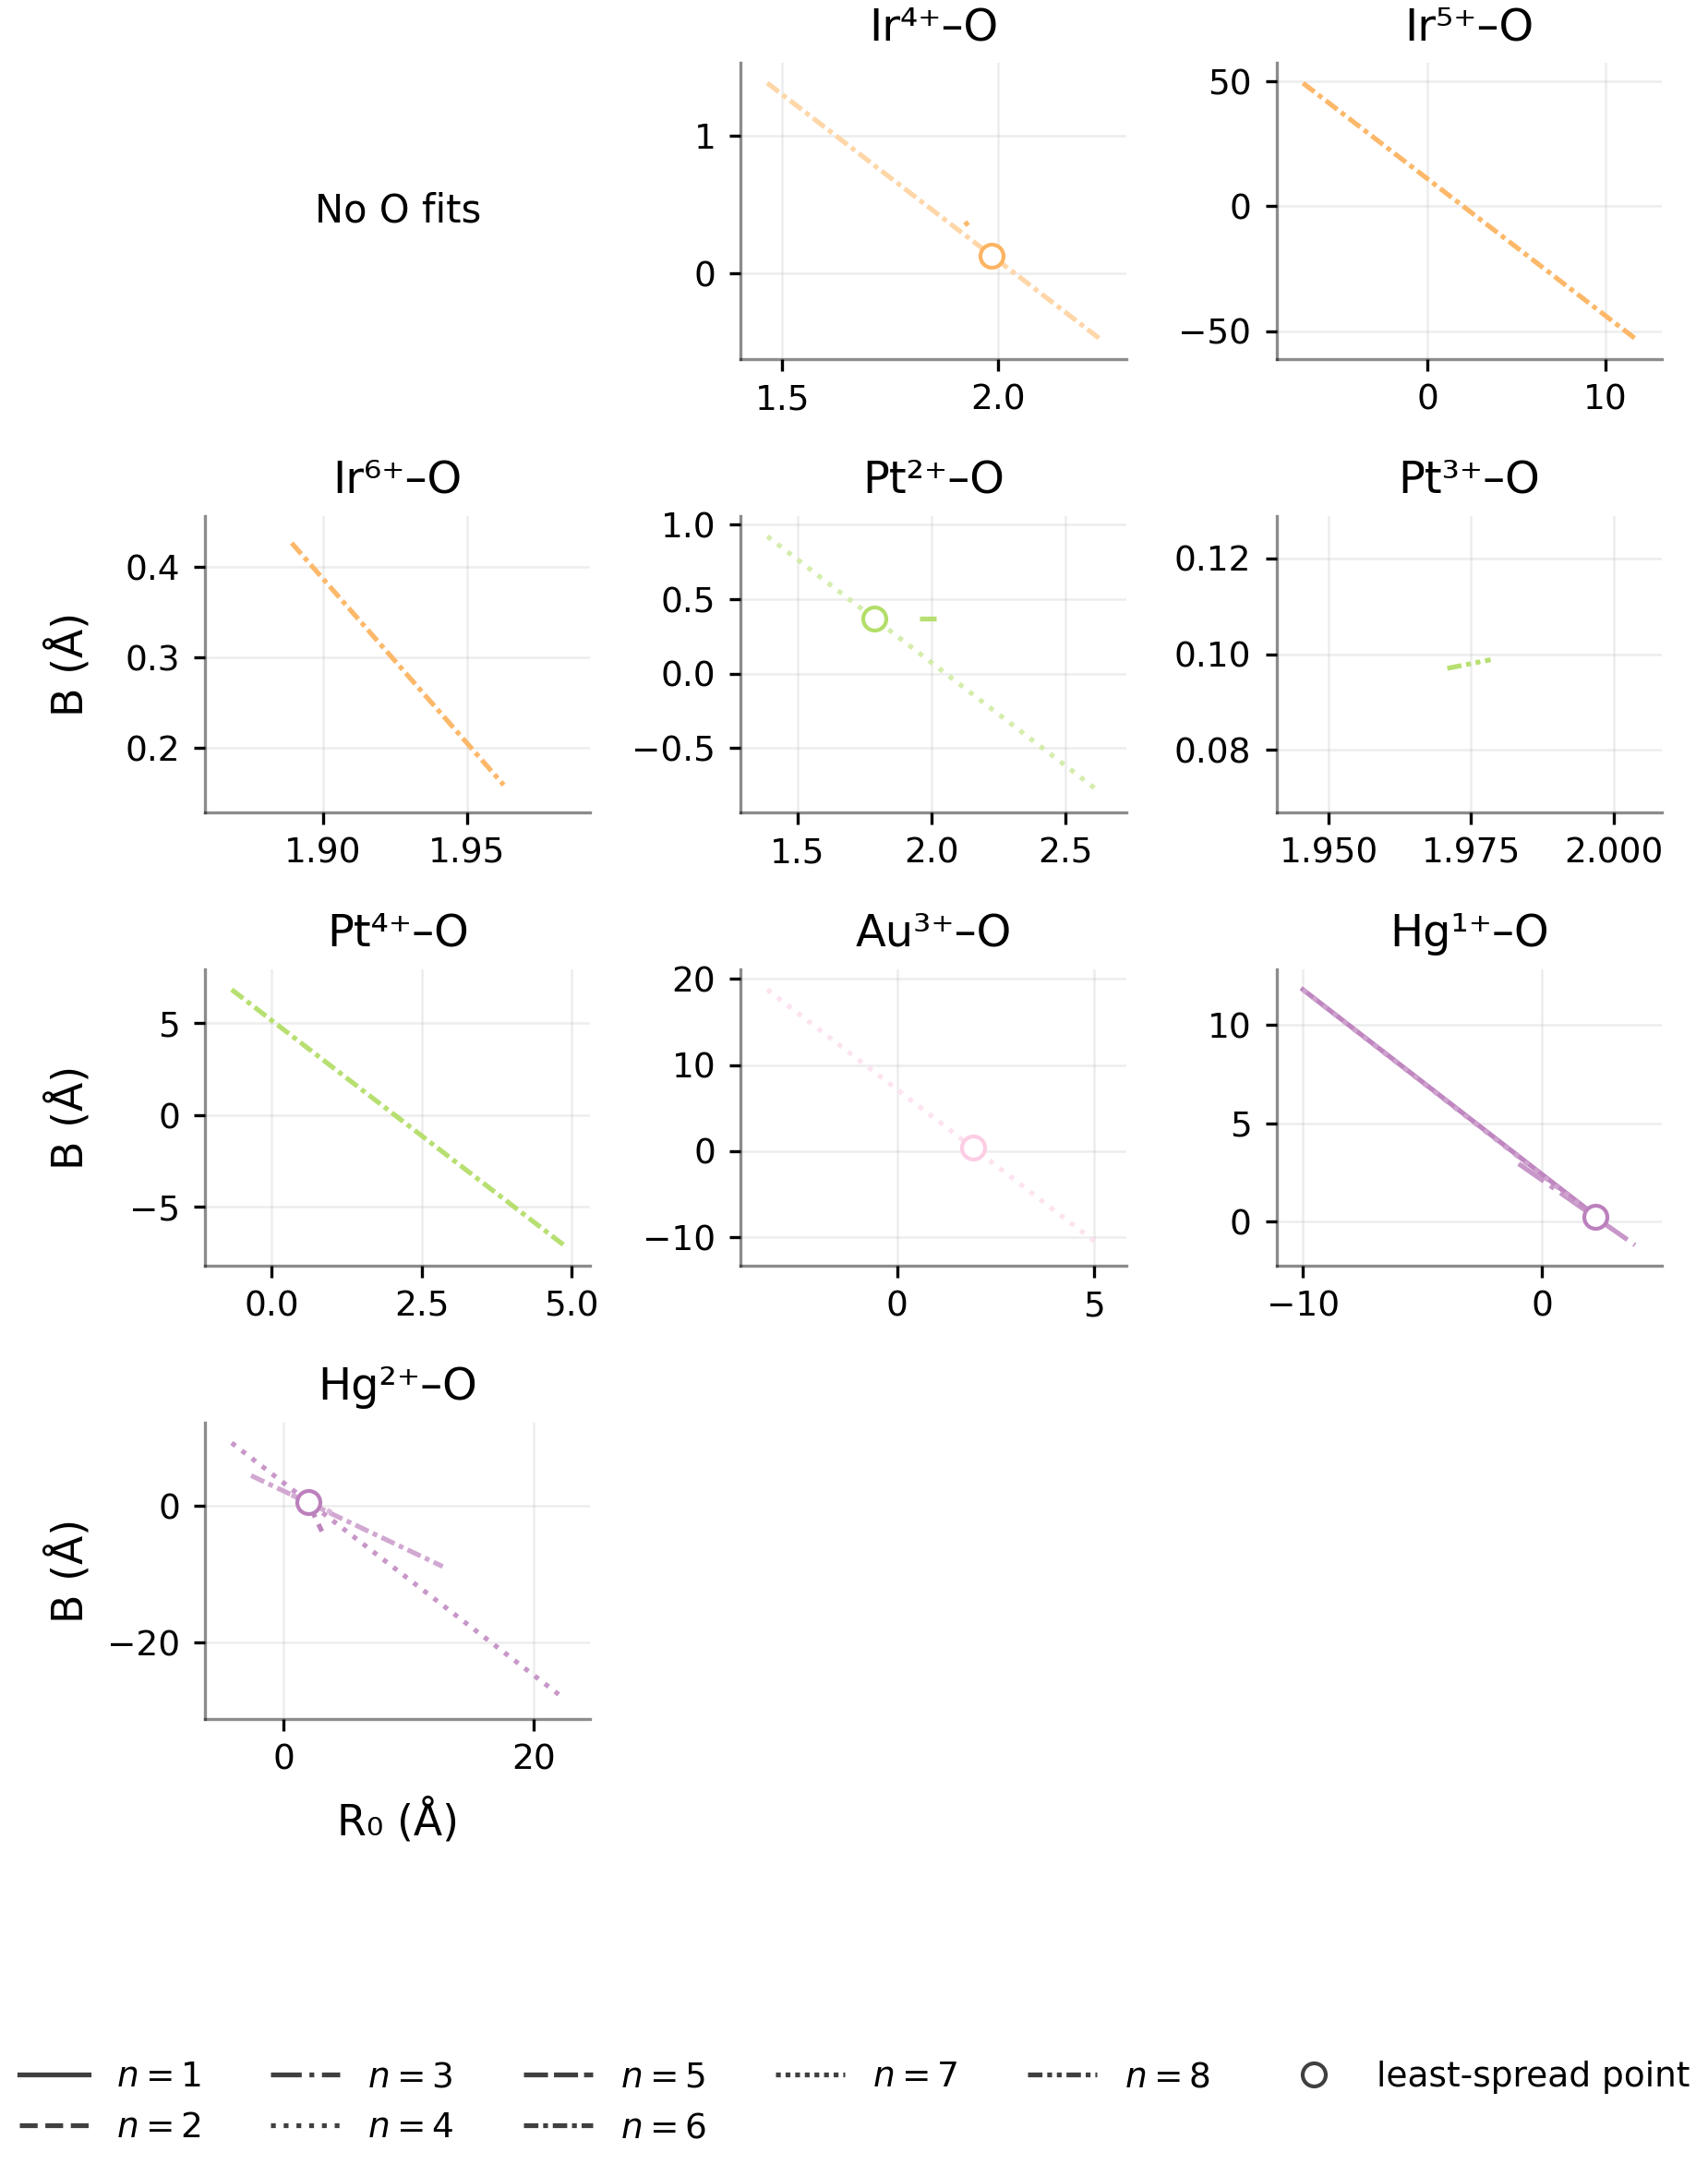
\includegraphics[width=\textwidth]{dblock_oxi_oxygen_cn_fit_lines_part08.png}
\caption{$n$-resolved $B$ vs.\ $R_0$ for oxidation-state--resolved 5$d$
X--O pairs (Ir--Hg).}
\label{fig:dblock_fits_8}
\end{figure}

\begin{figure}[p]
\centering
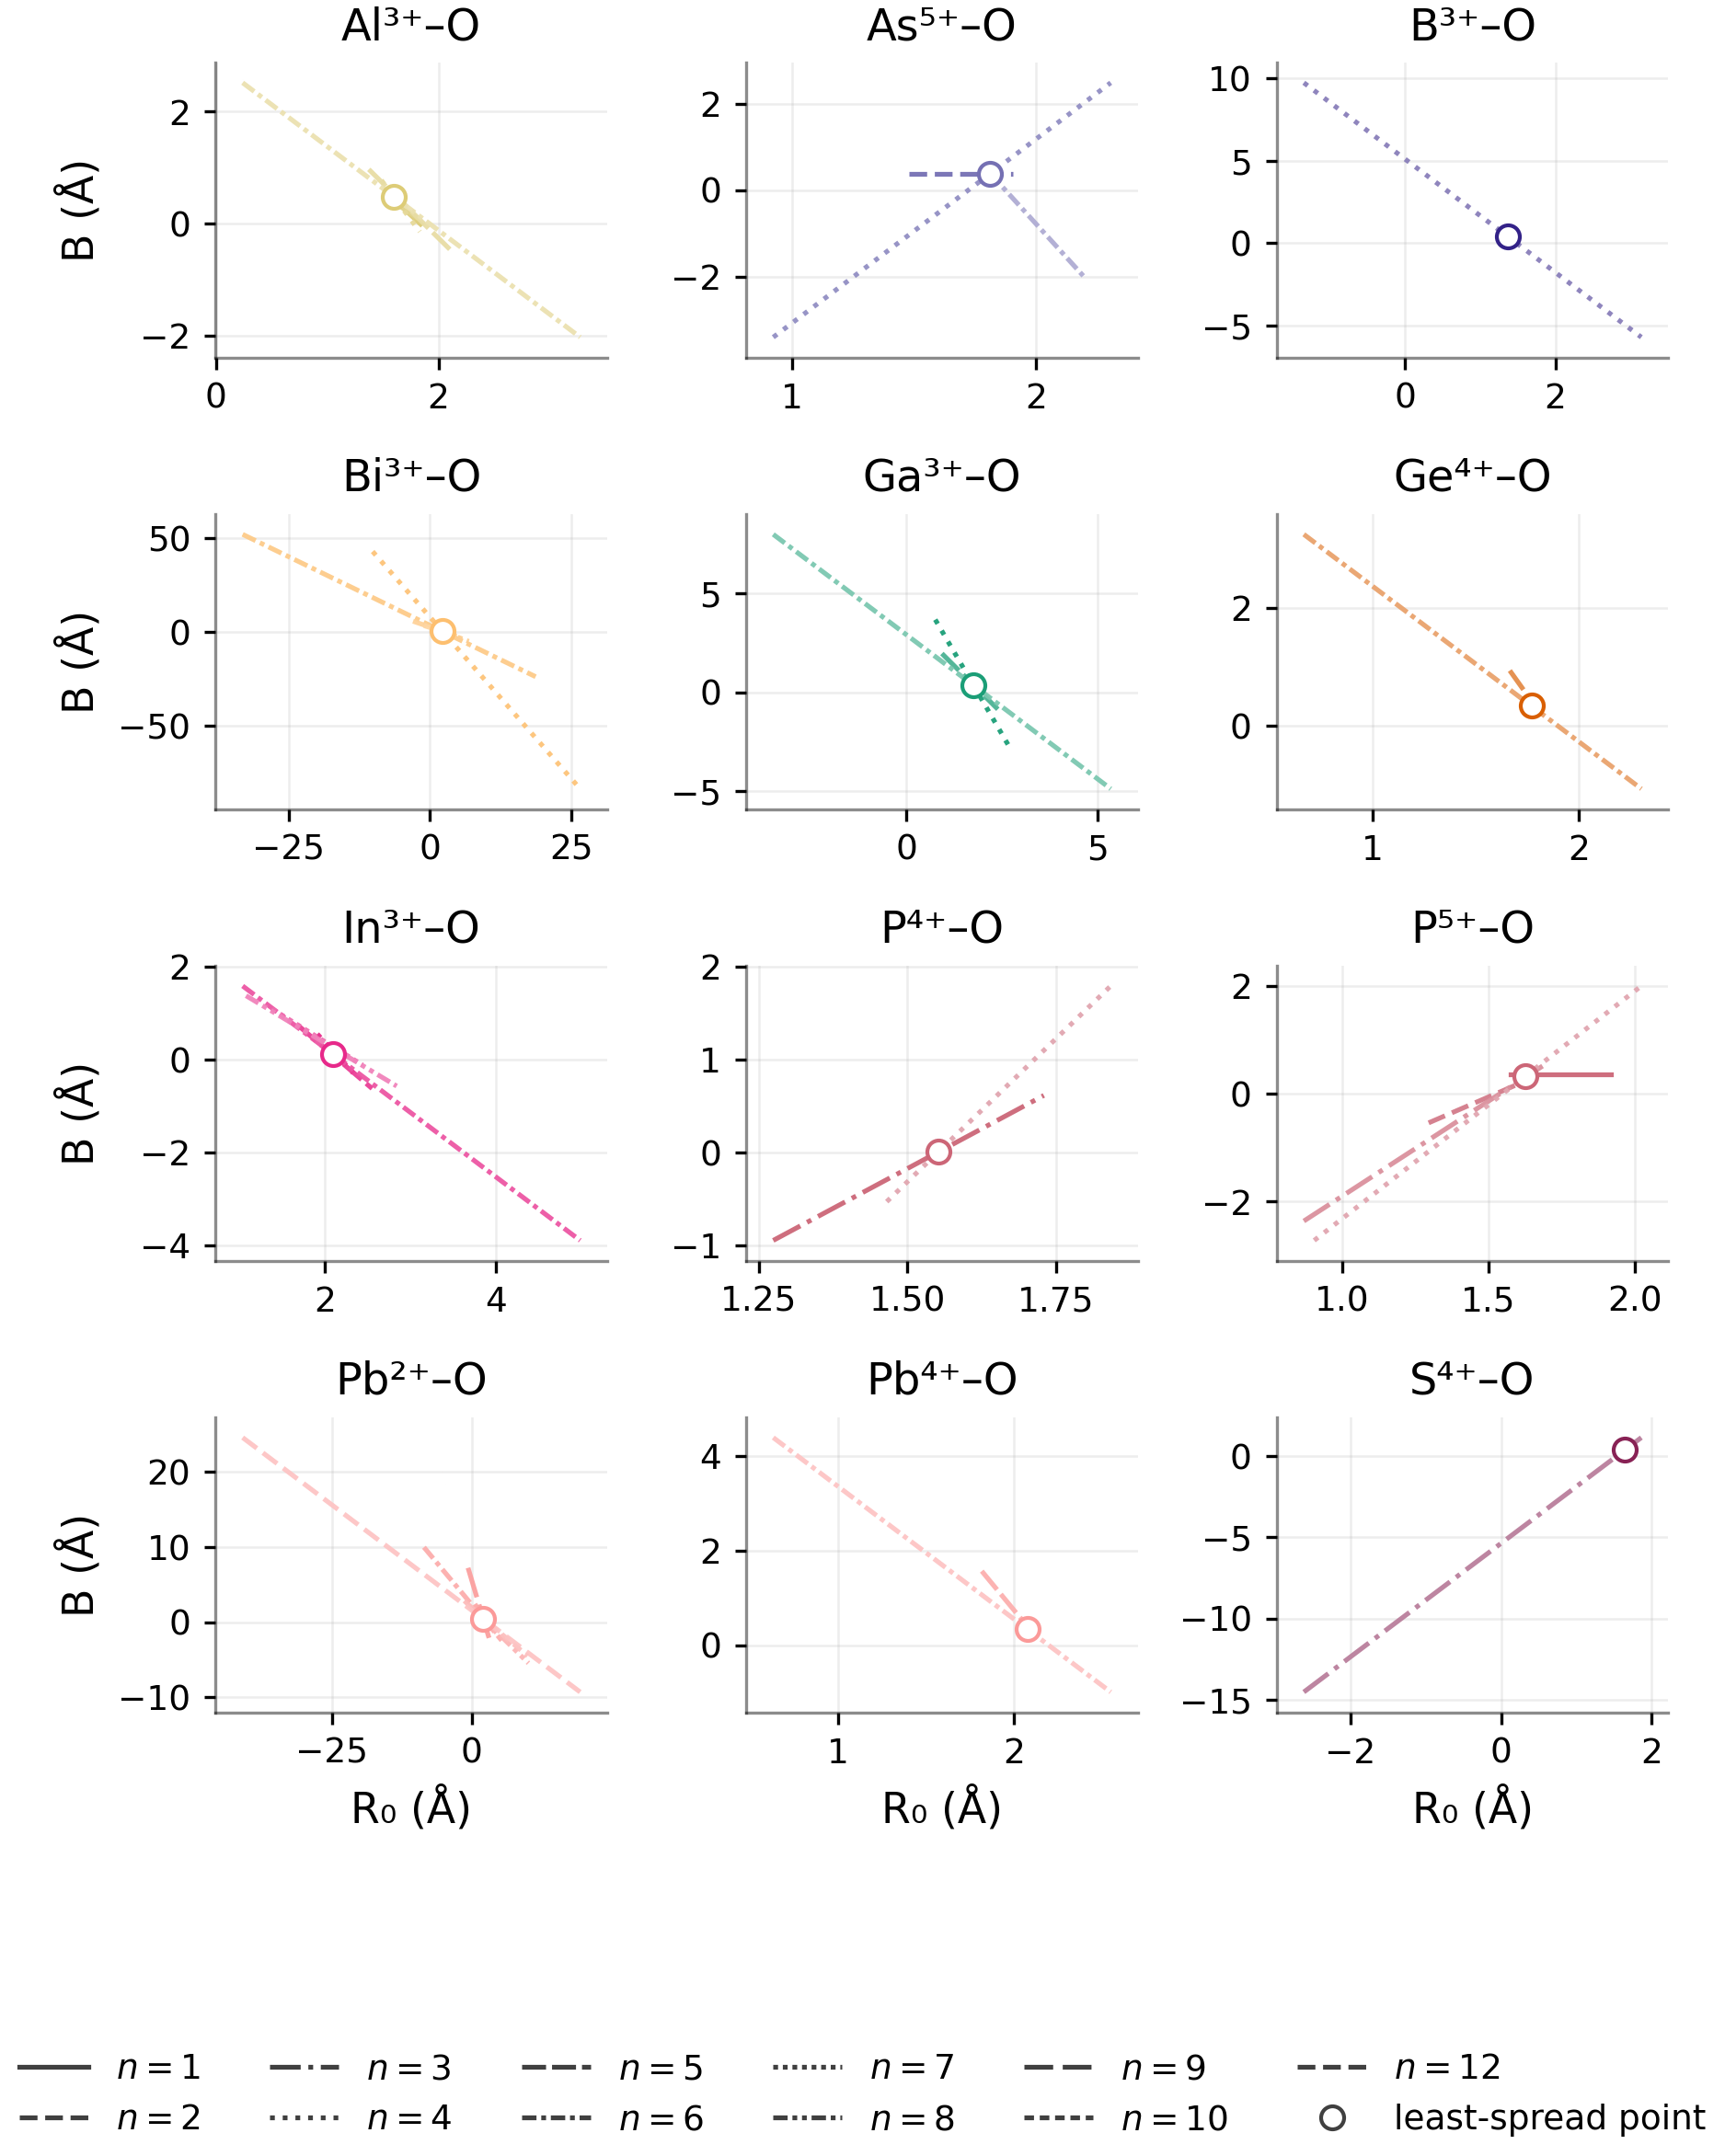
\includegraphics[width=0.95\textwidth]{pblock_oxygen_cn_fit_lines_part01.png}
\caption{$n$-resolved $B$ vs.\ $R_0$ for oxidation-state--resolved
$p$-block X--O pairs (Al$^{3+}$--S$^{4+}$).}
\label{fig:pblock_fits_1}
\end{figure}

\begin{figure}[p]
\centering
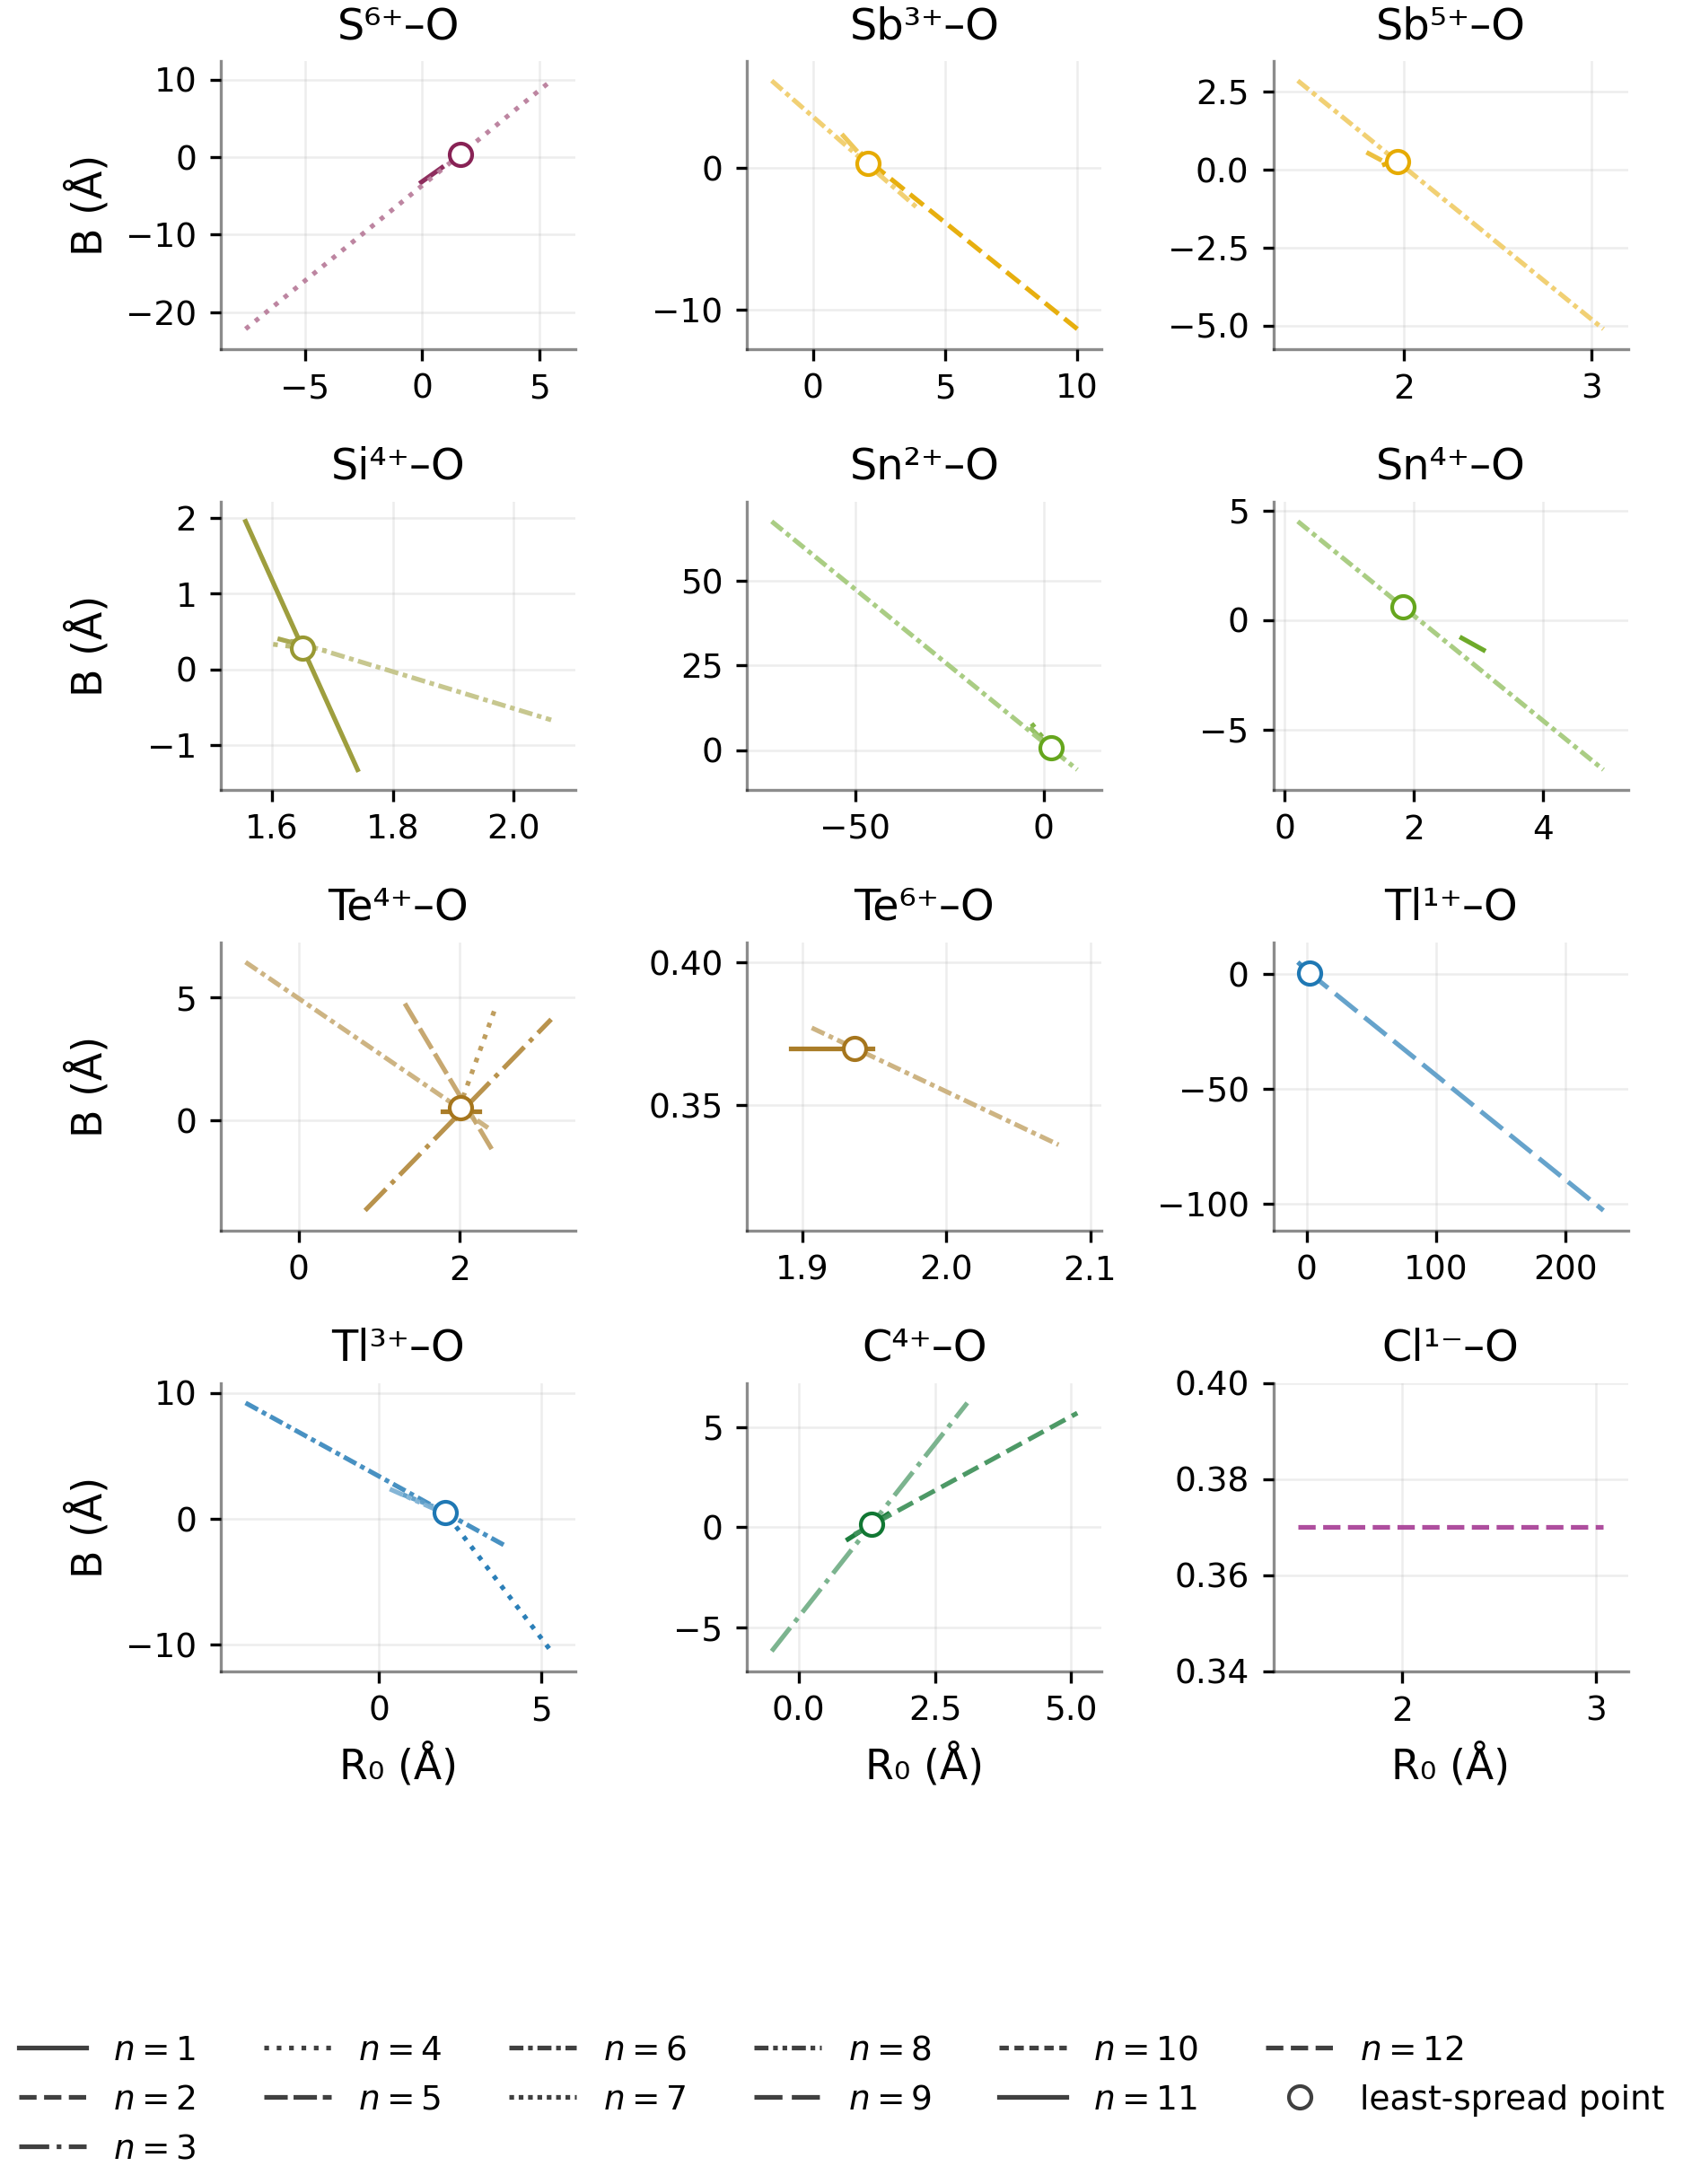
\includegraphics[width=0.95\textwidth]{pblock_oxygen_cn_fit_lines_part02.png}
\caption{$n$-resolved $B$ vs.\ $R_0$ for oxidation-state--resolved
$p$-block X--O pairs (S$^{6+}$--Cl).}
\label{fig:pblock_fits_2}
\end{figure}

\begin{figure}[p]
\centering
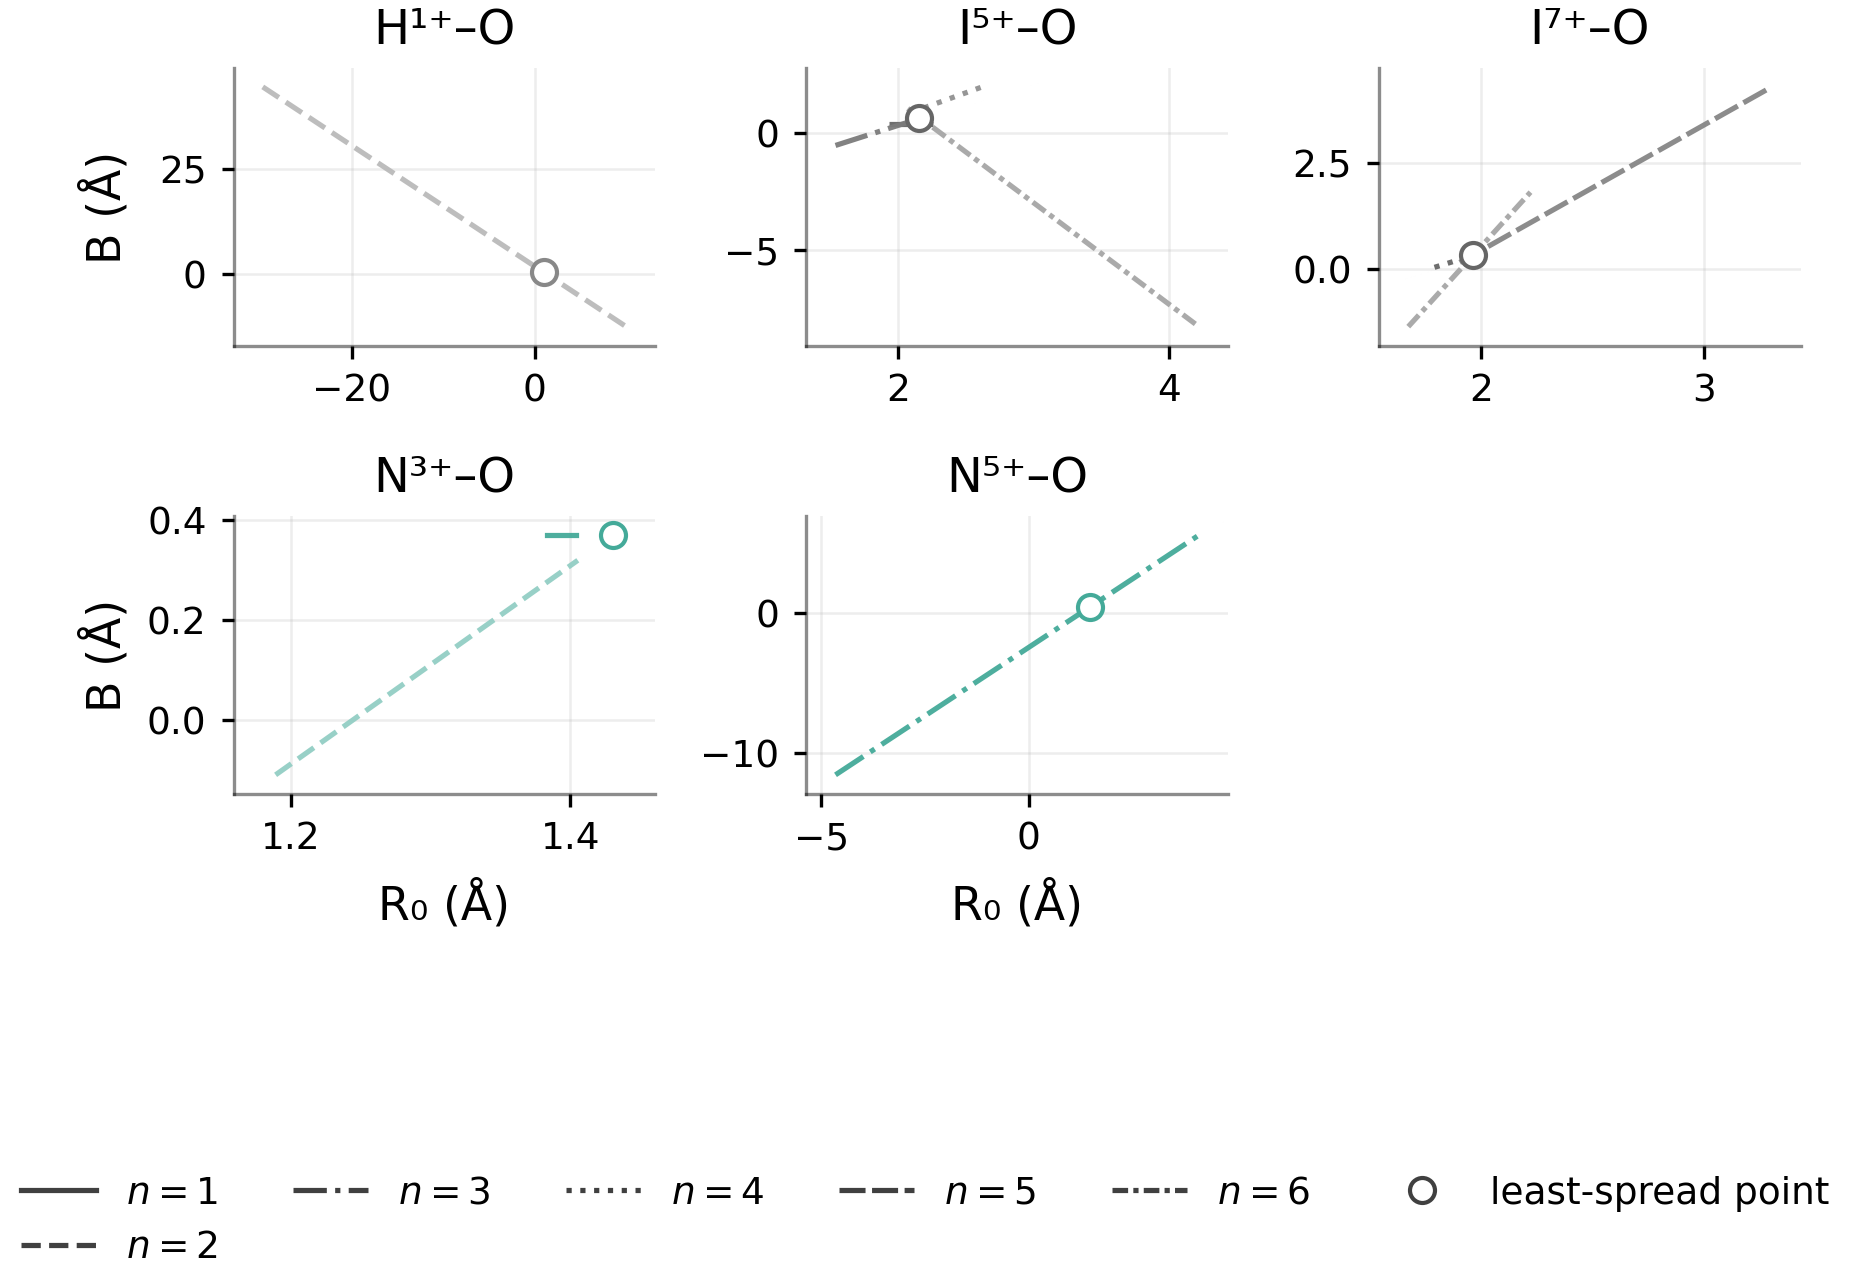
\includegraphics[width=0.95\textwidth]{pblock_oxygen_cn_fit_lines_part03.png}
\caption{$n$-resolved $B$ vs.\ $R_0$ for the remaining $p$-block and
hydrogen X--O pairs (H$^{1+}$, N$^{3+}$, N$^{5+}$, I$^{5+}$,
I$^{7+}$).}
\label{fig:pblock_fits_3}
\end{figure}

\begin{figure}[p]
\centering
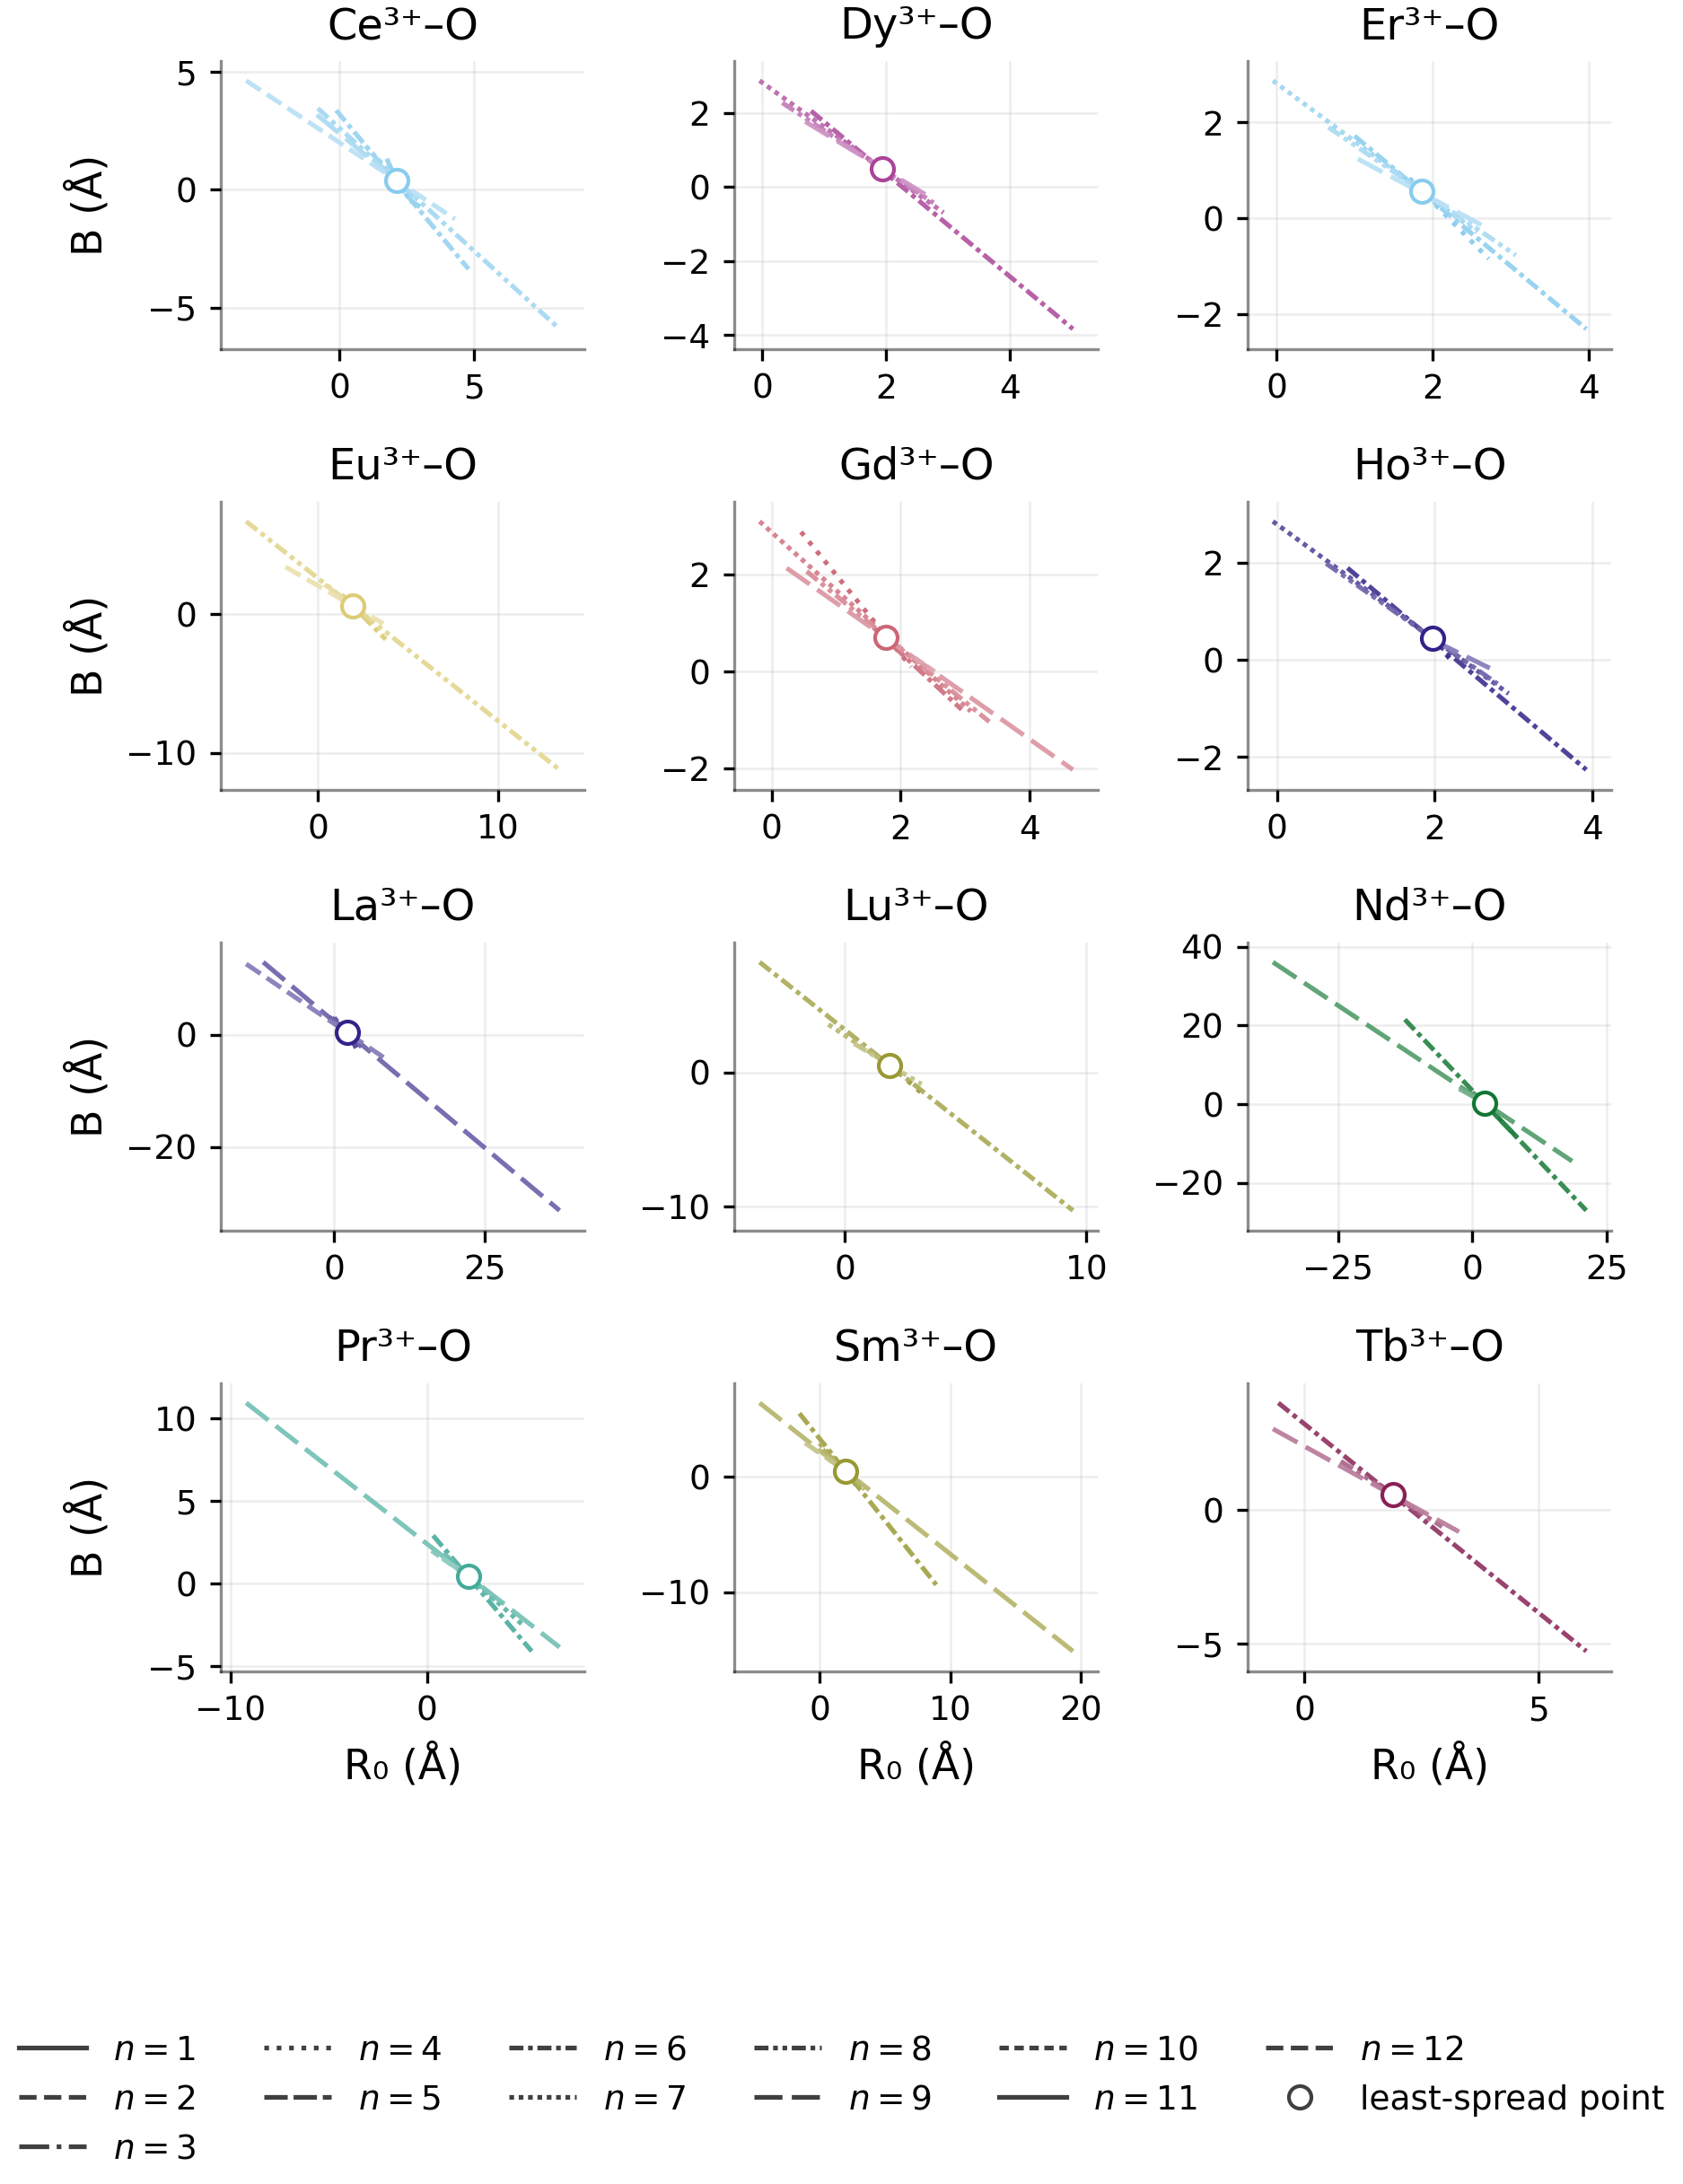
\includegraphics[width=0.95\textwidth]{fblock_oxygen_cn_fit_lines_part01.png}
\caption{$n$-resolved $B$ vs.\ $R_0$ for $f$-block trivalent
lanthanide X--O pairs (Ce$^{3+}$--Tb$^{3+}$).}
\label{fig:fblock_fits_1}
\end{figure}

\begin{figure}[p]
\centering
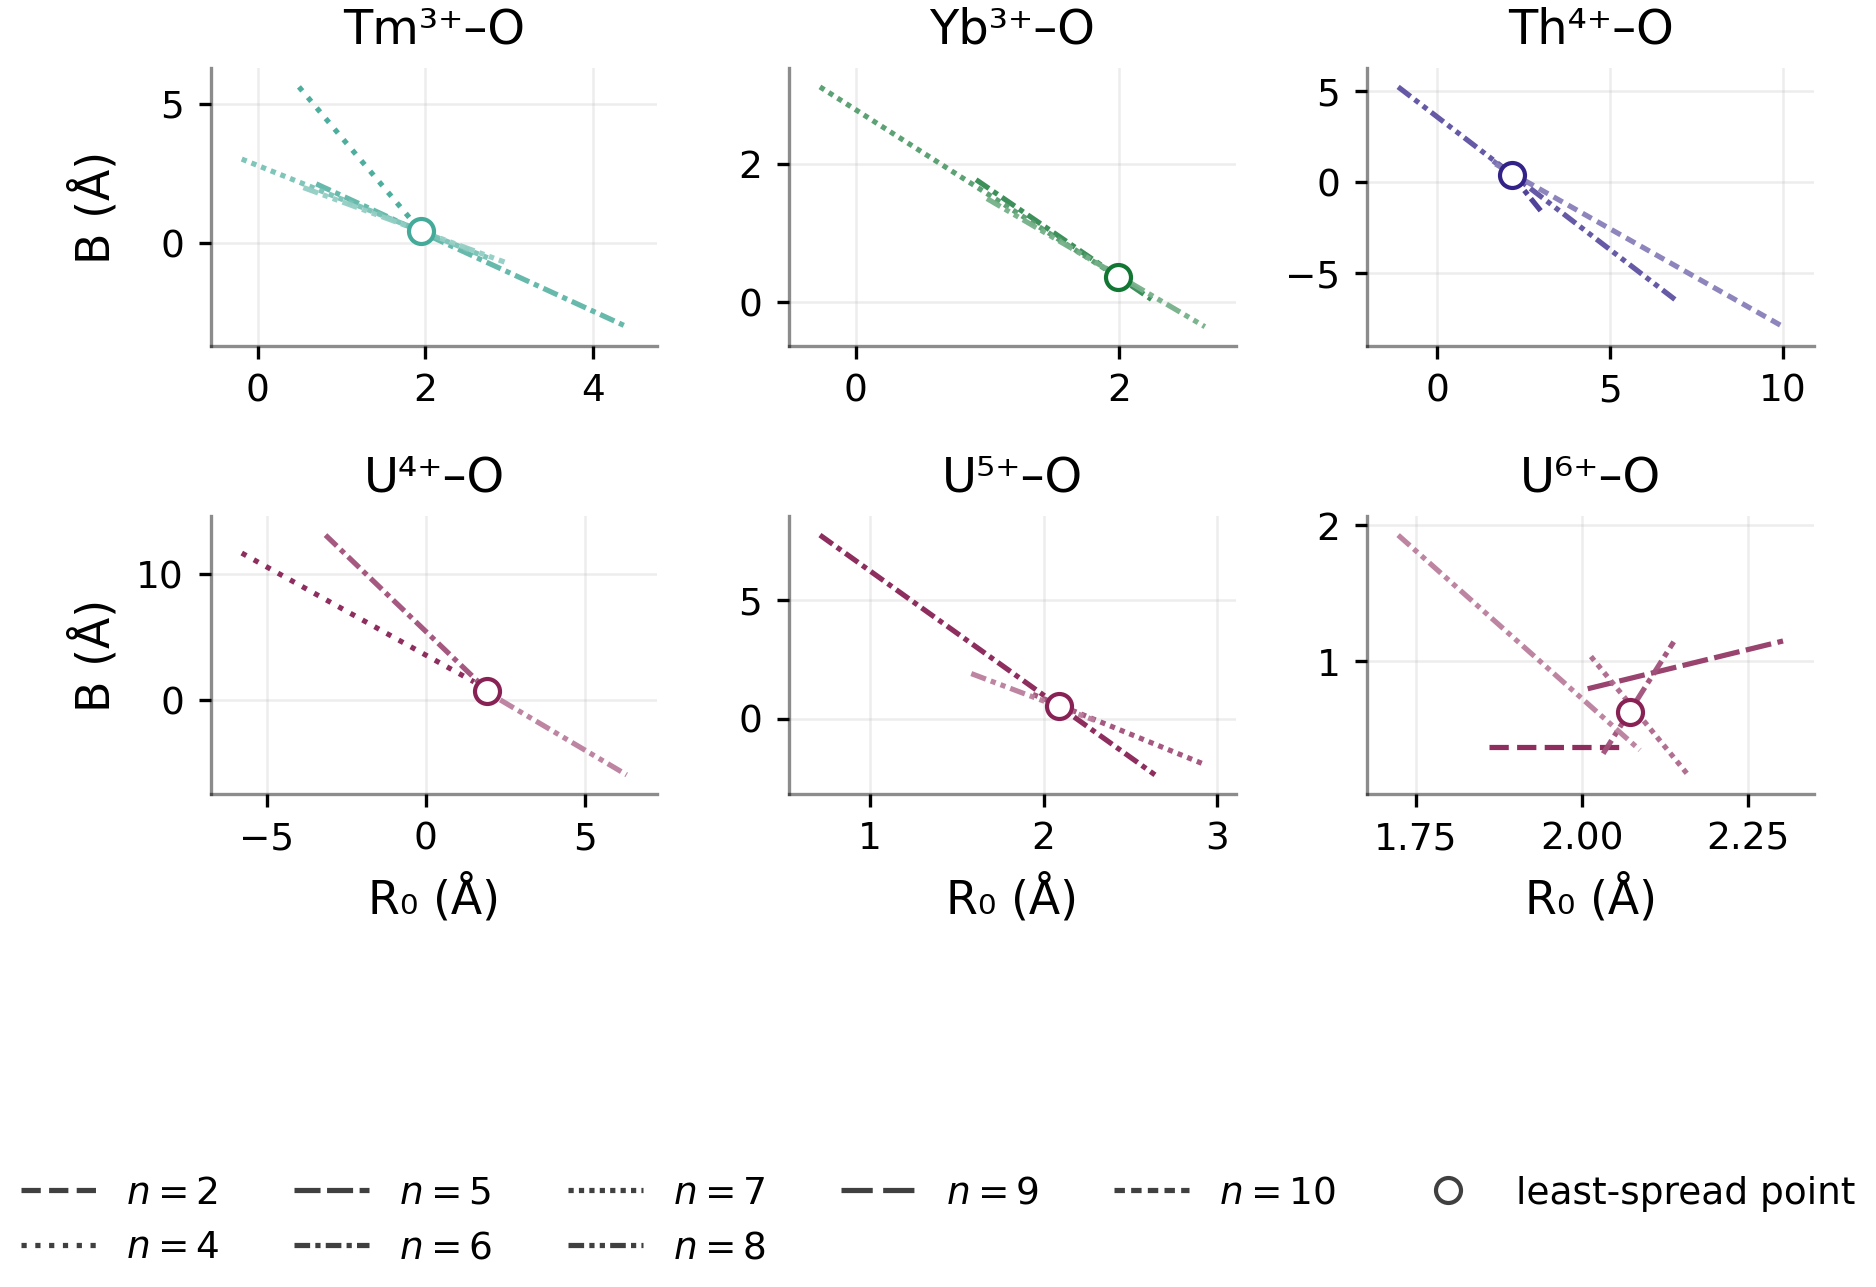
\includegraphics[width=0.95\textwidth]{fblock_oxygen_cn_fit_lines_part02.png}
\caption{$n$-resolved $B$ vs.\ $R_0$ for the remaining $f$-block
lanthanide and actinide X--O pairs (Tm$^{3+}$--Yb$^{3+}$ and
Th$^{4+}$--U$^{6+}$).}
\label{fig:fblock_fits_2}
\end{figure}

\clearpage

\section{Characteristic pairs and bond-length identity}

Figure~\ref{fig:r0star_bstar} shows the characteristic pairs
$(R_0^*,B^*)$ for Group~1 (including H$^+$), Group~2, and the
trivalent lanthanides.

For each species and coordination shell $n$, the fitted points define a
line $B=\beta^{(n)}R_0+\beta_0^{(n)}$.  The characteristic pair is the
weighted least-spread intersection of those $n$-resolved lines.  If the
final line fit for shell $n$ contains $N_n$ structures, we assign weight
$w_n=N_n$ and define the weighted means
\[
\bar\beta=\frac{\sum_n w_n\beta^{(n)}}{\sum_n w_n},
\qquad
\bar\beta_0=\frac{\sum_n w_n\beta_0^{(n)}}{\sum_n w_n}.
\]
The characteristic abscissa is then
\[
R_0^*=
-\frac{\sum_n w_n\bigl(\beta^{(n)}-\bar\beta\bigr)
\bigl(\beta_0^{(n)}-\bar\beta_0\bigr)}
{\sum_n w_n\bigl(\beta^{(n)}-\bar\beta\bigr)^2},
\]
which is the point that minimizes the weighted variance of the
line-by-line values $B_n(R_0)=\beta^{(n)}R_0+\beta_0^{(n)}$.  The
characteristic ordinate and its spread are
\[
B^*=
\frac{\sum_n w_n B_n(R_0^*)}{\sum_n w_n},
\qquad
\sigma_B=
\left[
\frac{\sum_n w_n\bigl(B_n(R_0^*)-B^*\bigr)^2}
{\sum_n w_n}
\right]^{1/2}.
\]
The tabulated $n_{\mathrm{CN}}$ counts how many distinct coordination
shells contribute to that intersection, while the weights entering the
intersection are the fitted structure counts in those shells.

\begin{figure}[t]
\centering
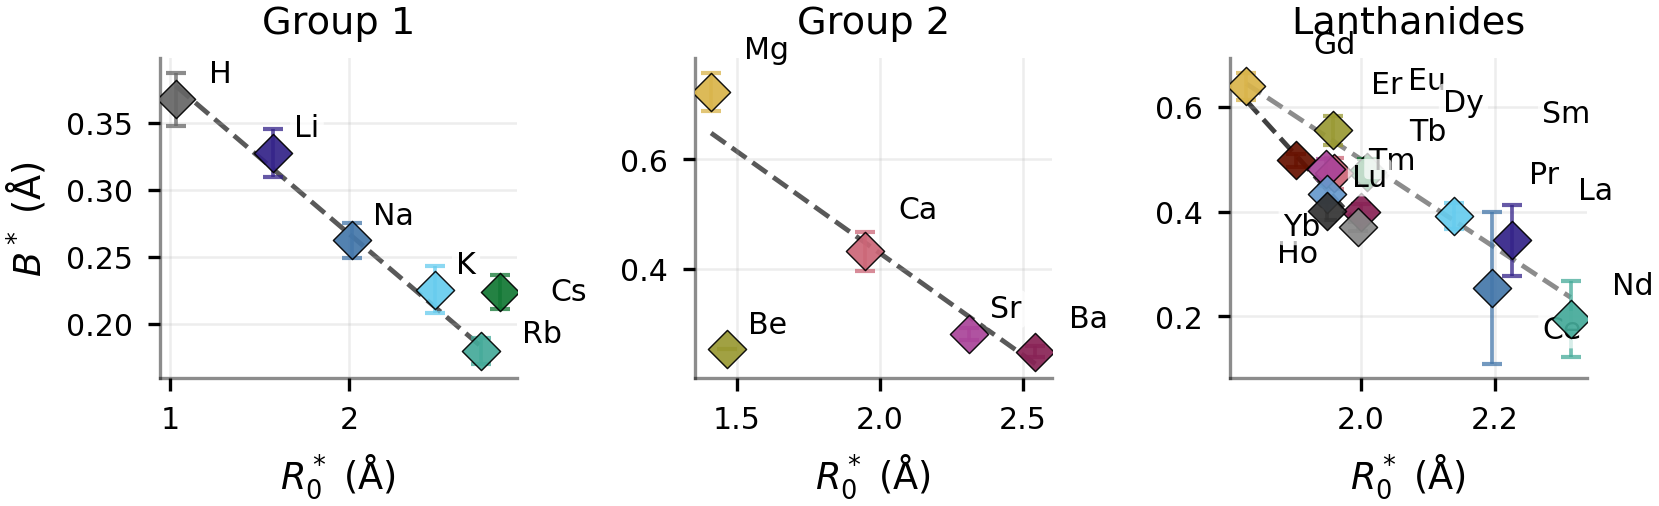
\includegraphics[width=0.85\textwidth]{group1_group2_lanthanide_r0_star_vs_b_star.png}
\caption[Characteristic pairs for Group~1, Group~2, and lanthanides.]{Characteristic $(R_0^*,B^*)$ for Group~1 including H$^+$
(left), Group~2 (center), and trivalent lanthanides (right).}
\label{fig:r0star_bstar}
\end{figure}

Figure~\ref{fig:identity} validates the bond-length identity
$R_0\approx\bar R+B\ln(z/n)$ across 50{,}706 cation--oxygen structures
(Pearson $r=0.969$, MAE$\,=0.018$~\AA).

\begin{figure}[t]
\centering
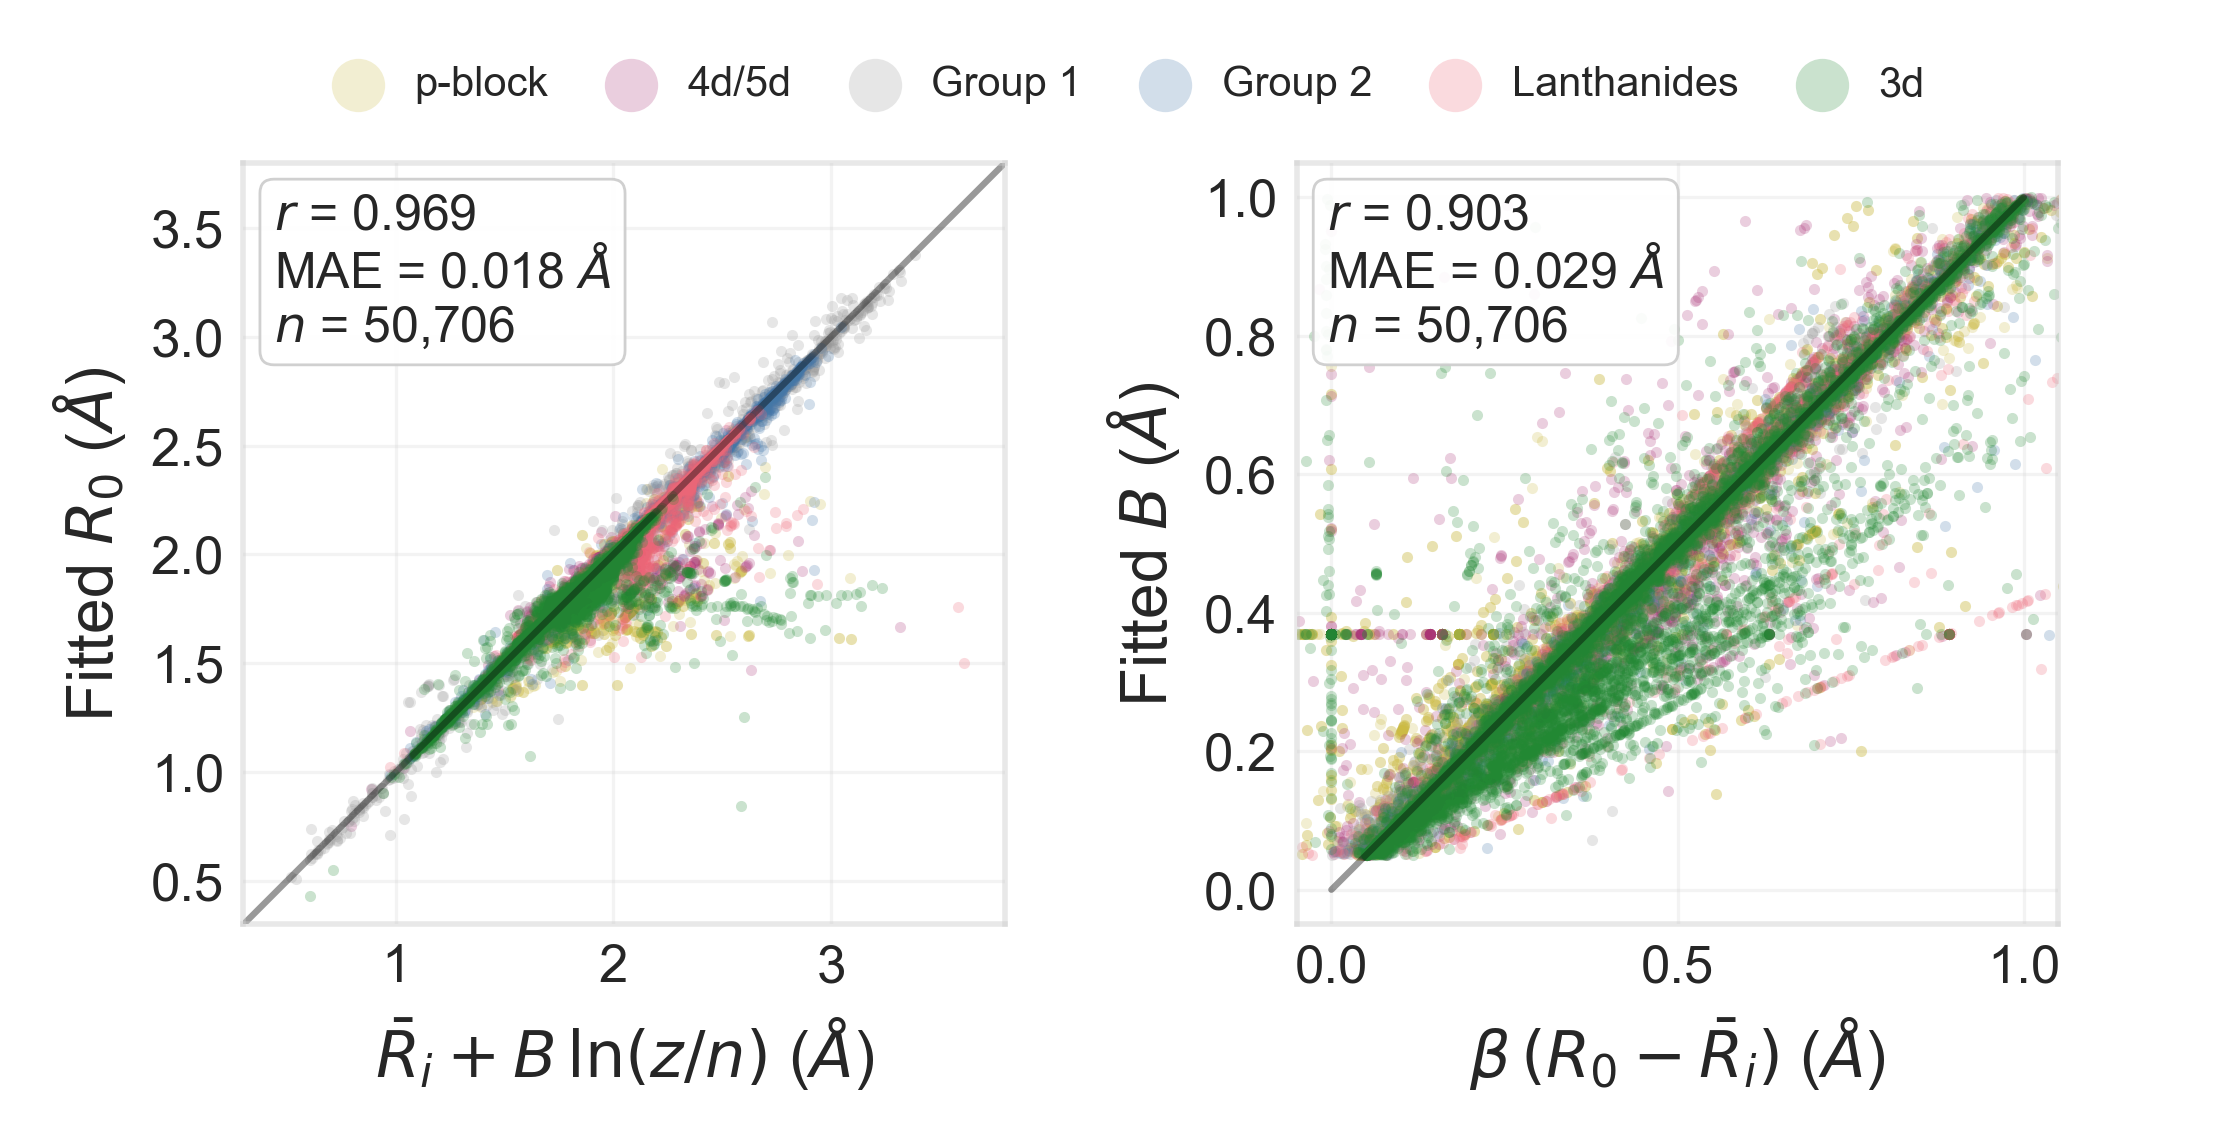
\includegraphics[width=0.85\textwidth]{r0_bond_length_identity_parity.png}
\caption[Bond-length-identity parity checks.]{Left: parity between fitted $R_0$ and $\bar R+B\ln(z/n)$ for
50{,}706 cation--oxygen structures.  Right: parity between fitted $B$
and $\beta(R_0-\bar R)$.}
\label{fig:identity}
\end{figure}

\section{\texorpdfstring{$s$-block screening-centroid controls}{s-block screening-centroid controls}}

For the ten Group~1/Group~2 ground-state binary oxides used in Fig.~2 of the
main text, the DFT screening centroid $r_{\mathrm{eff}}$ is compared
against three linear descriptors: the bond-valence shell centroid $m_i$,
the fitted bond-valence intercept $R_0$, and the Shannon cation radius.
Leave-one-out mean absolute errors are $0.006$~\AA\ for $m_i$,
$0.078$~\AA\ for $R_0$, and $0.094$~\AA\ for the Shannon-radius control,
showing that the $r_{\mathrm{eff}}$--$m_i$ collapse is substantially
sharper than a generic monotone size trend.

\begin{figure}[t]
\centering
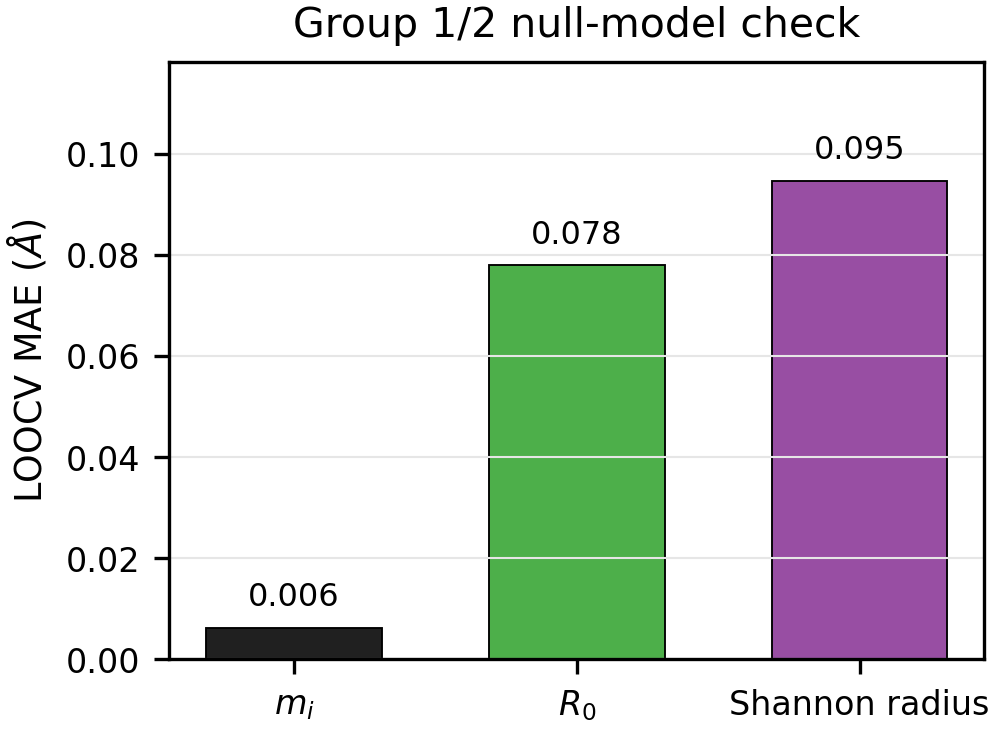
\includegraphics[width=0.55\textwidth]{thomas_fermi_reff_null_models_si.png}
\caption[Null-model check for the ten binary oxides.]{Leave-one-out null-model check for the ten Group~1/Group~2
binary oxides used in Fig.~2 of the main text.  Bars report the mean
absolute error of linear regressions against the bond-valence shell
centroid $m_i$, the fitted intercept $R_0$, and the Shannon cation radius.}
\label{fig:sblock_controls}
\end{figure}

Each oxide contributes one point $(m_i,r_{\mathrm{eff}})$ to
Fig.~2.  For a given oxide, the bond-valence shell centroid is computed
from the same fitted $(R_0,B)$ and coordination number $n$ used for its
bond-valence record, taking the $n$ shortest M--O distances in the
ground-state structure and forming
\[
p_{ij}=\frac{e^{-R_{ij}/B}}{\sum_{k=1}^n e^{-R_{ik}/B}},
\qquad
m_i=\sum_{j=1}^n p_{ij}R_{ij}.
\]
The DFT-side centroid is then built bond by bond over all oxygen
neighbors with $R_{ij}\le 3.5$~\AA.  Each such bond contributes one
oxygen-side path centroid
$r_{\mathrm{eff}}^{(\mathrm{path})}$, and the oxide-level
$r_{\mathrm{eff}}$ plotted in Fig.~2 is the simple arithmetic mean of
those finite bond-path centroids.

The offset in the main-text regression is quantified directly from that same
discrete bond-path construction.  Defining the oxygen-side pre-cusp valence centroid
shift by
\[
\Delta_{\mathrm{O,val}}:=\langle R_{ij}-r_{\mathrm{eff}}^{(\mathrm{path})}\rangle,
\]
let $\{r_g,\rho_g\}_{g=1}^{200}$ denote the total-density samples on the
nearest-image straight M--O segment at 200 uniformly spaced points.  The
bond critical-point proxy is the interior density minimum on the interval
$0.15R_{ij}<r<0.85R_{ij}$; denote its location and value by
$r_{\mathrm{BCP}}$ and $\rho_{\mathrm{BCP}}$.  The oxygen-side pre-cusp
window is the subset of sampled points with
$r_{\mathrm{BCP}}\le r_g\le 0.93R_{ij}$, finite $\rho_g$, and positive
finite Thomas--Fermi screening length $\lambda_{\mathrm{TF}}(\rho_g)$.
The Thomas--Fermi length enters here only as a positivity filter on the
sample window and does not appear in the centroid weights or in any of
the regression results; the \texttt{thomas\_fermi} tag in the
Fig.~2 file label reflects only the screening interpretation of
$r_{\mathrm{eff}}$, not its construction.
On that discrete window we use the excess-density weights
$w_g=\max[\rho_g-\rho_{\mathrm{BCP}},0]$; in the rare case that these
clipped weights vanish identically, we use $w_g=\rho_g$ instead.  Thus
\[
r_{\mathrm{eff}}^{(\mathrm{path})}=
\frac{\sum_g w_g r_g}{\sum_g w_g},
\]
and the oxide-level centroid used in Fig.~2 is the arithmetic mean of
$r_{\mathrm{eff}}^{(\mathrm{path})}$ over those first-shell M--O bonds.
No spline fitting, path relaxation, or topological bond-path search is
introduced beyond this fixed straight-segment sampling rule.  With that
definition, the ten-oxide $s$-block shift fit is
$\Delta_{\mathrm{O,val}} = 0.0613\,m_i + 0.2394$~\AA\
($R^2=0.963$), with mean $0.3910\pm0.0269$~\AA.  Equivalently,
$r_{\mathrm{eff}}=0.9387\,m_i-0.2394$~\AA, whose rounded form is the
main-text relation.  The intercept is therefore the zero-radius limit of
a directly measured oxygen-side screening shift, not an unconstrained
empirical parameter.

\paragraph*{Species-level screening length from the characteristic pair.}
The shell-level Yukawa inversion in the main text is written in terms of the
representative radius $R^*$, chosen operationally as the Boltzmann shell
centroid $m_i$.  To pass from that shell-level relation to a species-level
constant, we evaluate the inversion at the characteristic fixed point
$(R_0^*,B^*)$ on the characteristic reference shell defined by $m_i=R_0^*$.
Using the exact identity
\[
R_0 = m_i + B(\ln q_i - H_i),
\]
this reference-shell condition is equivalent at the fixed point to
$H_i=\ln q_i$, so the representative radius entering the Yukawa inversion is
$R^*=R_0^*$.  Substituting $B=B^*$ and $R^*=R_0^*$ into the positive screening
branch therefore gives
\[
\lambda^*=\frac{-R_0^*+\sqrt{R_0^{*2}+4B^*R_0^*}}{2},
\]
which is the species-level screening length reported in
Table~\ref{tab:lambda_star} for entries with $B^*>0$.

\section{Screening lengths for the analyzed species}

\begin{longtable}{l l r r r r}
\caption{Characteristic pairs $(R_0^*,B^*)$ for all 103 cation--oxygen
species and physical screening lengths $\lambda^*$ for the 101
screening-branch species, ordered by atomic number.  All values are in
\AA.  For entries with positive
characteristic ordinate ($B^*>0$), $\lambda^*$ is
computed from the screening-branch inversion in the main text;
$n_{\mathrm{CN}}$ is the number of distinct coordination shells used to
determine $(R_0^*,B^*)$.
Parenthetical uncertainties on $B^*$ are the weighted standard deviation
$\sigma_B$ of the $n$-resolved lines at $R_0^*$; uncertainties on
$\lambda^*$ are propagated for entries with $B^*>0$ via
$\sigma_\lambda=|\partial\lambda^*/\partial B^*|\,\sigma_B$.
Entries with $n_{\mathrm{CN}}=2$ have $\sigma_B=0$ by construction
and should be regarded as provisional.  Two species (Mo$^{3+}$ and
Sb$^{3+}$) yield $B^*<0$; these are retained as signed
Yukawa-branch diagnostics that the first-order expansion does not
adequately describe their bonding and are not assigned physical
$\lambda^*$ values.}
\label{tab:lambda_star} \\
\hline\hline
  Species & Block & $R_0^*$ & $B^*$ & $\lambda^*$ & $n_{\mathrm{CN}}$ \\
\hline
\endfirsthead
\multicolumn{6}{c}{\tablename\ \thetable{} -- continued from previous page} \\
\hline
  Species & Block & $R_0^*$ & $B^*$ & $\lambda^*$ & $n_{\mathrm{CN}}$ \\
\hline
\endhead
\hline
\multicolumn{6}{r}{Continued on next page} \\
\endfoot
\hline\hline
\endlastfoot
  H$^{1+}$             & $s$   & 1.026 &       0.369(9) &       0.288(6) & 9 \\
  Li$^{1+}$            & $s$   & 1.636 &      0.286(22) &      0.248(17) & 10 \\
  Be$^{2+}$            & $s$   & 1.452 &       0.272(0) &       0.234(0) & 2 \\
  B$^{3+}$             & $p$   & 1.376 &       0.372(9) &       0.304(6) & 7 \\
  C$^{4+}$             & $p$   & 1.337 &       0.135(4) &       0.123(3) & 3 \\
  N$^{3+}$             & $p$   & 1.431 &       0.370(0) &       0.305(0) & 2 \\
  N$^{5+}$             & $p$   & 1.492 &       0.437(0) &       0.354(0) & 2 \\
  Na$^{1+}$            & $s$   & 1.923 &      0.331(15) &      0.288(11) & 10 \\
  Mg$^{2+}$            & $s$   & 1.776 &      0.298(16) &      0.260(12) & 5 \\
  Al$^{3+}$            & $p$   & 1.648 &       0.407(9) &       0.338(6) & 6 \\
  Si$^{4+}$            & $p$   & 1.652 &       0.269(9) &       0.235(7) & 5 \\
  P$^{4+}$             & $p$   & 1.552 &       0.004(0) &       0.004(0) & 2 \\
  P$^{5+}$             & $p$   & 1.625 &       0.324(7) &       0.277(6) & 4 \\
  S$^{4+}$             & $p$   & 1.644 &       0.370(0) &       0.311(0) & 3 \\
  S$^{6+}$             & $p$   & 1.610 &       0.307(0) &       0.264(0) & 2 \\
  Cl$^{1-}$            & $p$   & 1.804 &       0.370(0) &       0.315(0) & 2 \\
  K$^{1+}$             & $s$   & 2.568 &      0.175(24) &      0.165(21) & 12 \\
  Ca$^{2+}$            & $s$   & 1.751 &      0.555(35) &      0.443(24) & 8 \\
  Sc$^{3+}$            & $d$   & 1.961 &      0.222(19) &      0.201(16) & 6 \\
  Ti$^{3+}$            & $d$   & 2.009 &       0.080(0) &       0.077(0) & 2 \\
  Ti$^{4+}$            & $d$   & 1.881 &      0.248(43) &      0.222(35) & 6 \\
  V$^{3+}$             & $d$   & 1.782 &      0.375(22) &      0.318(16) & 6 \\
  V$^{4+}$             & $d$   & 1.821 &      0.353(15) &      0.303(11) & 5 \\
  V$^{5+}$             & $d$   & 1.849 &      0.448(75) &      0.373(53) & 6 \\
  Cr$^{2+}$            & $d$   & 1.744 &      0.435(14) &      0.360(10) & 3 \\
  Cr$^{3+}$            & $d$   & 1.761 &       0.370(0) &       0.314(0) & 3 \\
  Cr$^{4+}$            & $d$   & 1.665 &       0.670(0) &       0.512(0) & 2 \\
  Cr$^{5+}$            & $d$   & 1.821 &      0.544(93) &      0.439(63) & 3 \\
  Mn$^{2+}$            & $d$   & 1.830 &       0.354(6) &       0.304(5) & 7 \\
  Mn$^{3+}$            & $d$   & 1.810 &      0.357(18) &      0.305(13) & 7 \\
  Mn$^{4+}$            & $d$   & 1.830 &       0.296(0) &       0.260(0) & 2 \\
  Fe$^{2+}$            & $d$   & 1.760 &      0.385(22) &      0.325(16) & 6 \\
  Fe$^{3+}$            & $d$   & 1.799 &       0.352(9) &       0.302(6) & 5 \\
  Fe$^{4+}$            & $d$   & 1.816 &       0.394(0) &       0.333(0) & 2 \\
  Co$^{1+}$            & $d$   & 1.584 &       0.370(0) &       0.310(0) & 2 \\
  Co$^{2+}$            & $d$   & 1.712 &       0.384(6) &       0.323(5) & 4 \\
  Co$^{3+}$            & $d$   & 1.776 &       0.354(5) &       0.303(3) & 4 \\
  Co$^{4+}$            & $d$   & 1.774 &      0.330(38) &      0.284(29) & 3 \\
  Ni$^{2+}$            & $d$   & 1.766 &       0.304(8) &       0.264(6) & 5 \\
  Ni$^{3+}$            & $d$   & 1.773 &      0.364(12) &       0.310(9) & 3 \\
  Cu$^{1+}$            & $d$   & 1.585 &      0.319(53) &      0.273(40) & 4 \\
  Cu$^{2+}$            & $d$   & 1.715 &      0.358(36) &      0.304(27) & 7 \\
  Cu$^{3+}$            & $d$   & 1.708 &      0.481(42) &      0.391(29) & 3 \\
  Zn$^{2+}$            & $d$   & 1.760 &       0.328(7) &       0.283(5) & 4 \\
  Ga$^{3+}$            & $p$   & 1.756 &       0.357(5) &       0.304(4) & 4 \\
  Ge$^{4+}$            & $p$   & 1.771 &      0.354(15) &      0.302(11) & 4 \\
  As$^{5+}$            & $p$   & 1.812 &       0.382(1) &       0.324(1) & 3 \\
  Rb$^{1+}$            & $s$   & 2.809 &      0.146(16) &      0.140(15) & 10 \\
  Sr$^{2+}$            & $s$   & 2.317 &      0.279(17) &      0.252(14) & 9 \\
  Y$^{3+}$             & $d$   & 1.806 &      0.634(18) &      0.497(12) & 9 \\
  Zr$^{4+}$            & $d$   & 1.979 &      0.330(27) &      0.288(21) & 6 \\
  Nb$^{5+}$            & $d$   & 1.945 &      0.426(30) &      0.359(22) & 7 \\
  Mo$^{3+}$            & $d$   & 2.324 &    $-$0.237(0) &            --- & 2 \\
  Mo$^{5+}$            & $d$   & 1.919 &      0.415(46) &      0.351(34) & 4 \\
  Mo$^{6+}$            & $d$   & 1.948 &      0.368(19) &      0.317(14) & 5 \\
  Pd$^{2+}$            & $d$   & 1.402 &       0.918(0) &       0.632(0) & 2 \\
  Ag$^{1+}$            & $d$   & 2.477 &      0.011(61) &      0.011(60) & 8 \\
  Ag$^{2+}$            & $d$   & 1.778 &       0.548(0) &       0.439(0) & 2 \\
  Cd$^{2+}$            & $d$   & 2.083 &      0.247(18) &      0.223(15) & 6 \\
  In$^{3+}$            & $p$   & 2.065 &      0.162(34) &      0.151(30) & 5 \\
  Sn$^{2+}$            & $p$   & 1.903 &      0.607(45) &      0.484(30) & 4 \\
  Sn$^{4+}$            & $p$   & 1.845 &       0.567(9) &       0.455(6) & 3 \\
  Sb$^{3+}$            & $p$   & 2.434 &   $-$0.341(87) &            --- & 5 \\
  Sb$^{5+}$            & $p$   & 1.990 &      0.130(39) &      0.122(35) & 4 \\
  Te$^{4+}$            & $p$   & 2.023 &     0.562(151) &     0.458(104) & 7 \\
  Te$^{6+}$            & $p$   & 1.937 &       0.370(0) &       0.318(0) & 2 \\
  I$^{5+}$             & $p$   & 2.077 &      0.476(34) &      0.399(24) & 6 \\
  I$^{7+}$             & $p$   & 1.964 &       0.324(4) &       0.283(3) & 3 \\
  Cs$^{1+}$            & $s$   & 2.921 &      0.185(21) &      0.175(19) & 11 \\
  Ba$^{2+}$            & $s$   & 2.453 &      0.308(11) &       0.277(9) & 10 \\
  La$^{3+}$            & $f$   & 2.171 &      0.404(41) &      0.348(31) & 12 \\
  Ce$^{3+}$            & $f$   & 2.142 &      0.360(50) &      0.314(39) & 9 \\
  Pr$^{3+}$            & $f$   & 2.112 &      0.427(30) &      0.364(22) & 7 \\
  Nd$^{3+}$            & $f$   & 2.307 &      0.207(50) &      0.191(43) & 8 \\
  Sm$^{3+}$            & $f$   & 1.971 &      0.522(13) &       0.429(9) & 8 \\
  Eu$^{3+}$            & $f$   & 2.088 &      0.396(28) &      0.340(21) & 6 \\
  Gd$^{3+}$            & $f$   & 1.784 &      0.688(28) &      0.530(17) & 6 \\
  Tb$^{3+}$            & $f$   & 1.862 &      0.598(18) &      0.476(12) & 5 \\
  Dy$^{3+}$            & $f$   & 1.938 &      0.486(18) &      0.403(13) & 5 \\
  Ho$^{3+}$            & $f$   & 1.967 &      0.444(16) &      0.373(11) & 5 \\
  Er$^{3+}$            & $f$   & 1.854 &      0.564(10) &       0.453(7) & 5 \\
  Tm$^{3+}$            & $f$   & 1.946 &      0.436(18) &      0.367(13) & 4 \\
  Yb$^{3+}$            & $f$   & 1.995 &       0.372(7) &       0.321(5) & 4 \\
  Lu$^{3+}$            & $f$   & 1.863 &      0.515(13) &       0.420(9) & 5 \\
  Hf$^{4+}$            & $d$   & 1.929 &      0.362(16) &      0.311(12) & 4 \\
  Ta$^{5+}$            & $d$   & 1.924 &      0.400(14) &      0.340(10) & 5 \\
  W$^{6+}$             & $d$   & 1.936 &      0.305(20) &      0.268(15) & 4 \\
  Re$^{6+}$            & $d$   & 1.928 &       0.363(0) &       0.312(0) & 2 \\
  Re$^{7+}$            & $d$   & 1.948 &      0.377(72) &      0.323(54) & 4 \\
  Ir$^{4+}$            & $d$   & 1.984 &       0.133(0) &       0.125(0) & 2 \\
  Pt$^{2+}$            & $d$   & 1.785 &       0.370(0) &       0.315(0) & 2 \\
  Au$^{3+}$            & $d$   & 1.924 &      0.363(13) &      0.312(10) & 3 \\
  Hg$^{1+}$            & $d$   & 2.230 &      0.233(28) &      0.213(24) & 4 \\
  Hg$^{2+}$            & $d$   & 1.929 &     0.605(122) &      0.484(81) & 6 \\
  Tl$^{1+}$            & $p$   & 2.459 &      0.272(19) &      0.247(16) & 10 \\
  Tl$^{3+}$            & $p$   & 2.054 &      0.469(42) &      0.394(30) & 4 \\
  Pb$^{2+}$            & $p$   & 2.240 &      0.348(31) &      0.306(24) & 10 \\
  Pb$^{4+}$            & $p$   & 2.080 &      0.353(23) &      0.308(17) & 3 \\
  Bi$^{3+}$            & $p$   & 2.104 &      0.430(31) &      0.366(23) & 8 \\
  Th$^{4+}$            & $f$   & 2.128 &      0.459(26) &      0.388(19) & 5 \\
  U$^{4+}$             & $f$   & 1.938 &      0.787(91) &      0.600(56) & 3 \\
  U$^{5+}$             & $f$   & 2.089 &      0.521(23) &      0.431(16) & 3 \\
  U$^{6+}$             & $f$   & 2.080 &      0.603(92) &      0.489(63) & 7 \\
\end{longtable}


\bibliography{references}

\end{document}
